% Options for packages loaded elsewhere
\PassOptionsToPackage{unicode}{hyperref}
\PassOptionsToPackage{hyphens}{url}
\PassOptionsToPackage{dvipsnames,svgnames,x11names}{xcolor}
\documentclass[
]{article}
\usepackage{xcolor}
\usepackage[margin=1in]{geometry}
\usepackage{amsmath,amssymb}
\setcounter{secnumdepth}{5}
\usepackage{iftex}
\ifPDFTeX
  \usepackage[T1]{fontenc}
  \usepackage[utf8]{inputenc}
  \usepackage{textcomp} % provide euro and other symbols
\else % if luatex or xetex
  \usepackage{unicode-math} % this also loads fontspec
  \defaultfontfeatures{Scale=MatchLowercase}
  \defaultfontfeatures[\rmfamily]{Ligatures=TeX,Scale=1}
\fi
\usepackage{lmodern}
\ifPDFTeX\else
  % xetex/luatex font selection
  \setmainfont[]{true}
  \setsansfont[]{Lato}
  \setmonofont[]{JetBrains Mono}
\fi
% Use upquote if available, for straight quotes in verbatim environments
\IfFileExists{upquote.sty}{\usepackage{upquote}}{}
\IfFileExists{microtype.sty}{% use microtype if available
  \usepackage[]{microtype}
  \UseMicrotypeSet[protrusion]{basicmath} % disable protrusion for tt fonts
}{}
\makeatletter
\@ifundefined{KOMAClassName}{% if non-KOMA class
  \IfFileExists{parskip.sty}{%
    \usepackage{parskip}
  }{% else
    \setlength{\parindent}{0pt}
    \setlength{\parskip}{6pt plus 2pt minus 1pt}}
}{% if KOMA class
  \KOMAoptions{parskip=half}}
\makeatother
\usepackage{color}
\usepackage{fancyvrb}
\newcommand{\VerbBar}{|}
\newcommand{\VERB}{\Verb[commandchars=\\\{\}]}
\DefineVerbatimEnvironment{Highlighting}{Verbatim}{commandchars=\\\{\}}
% Add ',fontsize=\small' for more characters per line
\usepackage{framed}
\definecolor{shadecolor}{RGB}{248,248,248}
\newenvironment{Shaded}{\begin{snugshade}}{\end{snugshade}}
\newcommand{\AlertTok}[1]{\textcolor[rgb]{0.94,0.16,0.16}{#1}}
\newcommand{\AnnotationTok}[1]{\textcolor[rgb]{0.56,0.35,0.01}{\textbf{\textit{#1}}}}
\newcommand{\AttributeTok}[1]{\textcolor[rgb]{0.13,0.29,0.53}{#1}}
\newcommand{\BaseNTok}[1]{\textcolor[rgb]{0.00,0.00,0.81}{#1}}
\newcommand{\BuiltInTok}[1]{#1}
\newcommand{\CharTok}[1]{\textcolor[rgb]{0.31,0.60,0.02}{#1}}
\newcommand{\CommentTok}[1]{\textcolor[rgb]{0.56,0.35,0.01}{\textit{#1}}}
\newcommand{\CommentVarTok}[1]{\textcolor[rgb]{0.56,0.35,0.01}{\textbf{\textit{#1}}}}
\newcommand{\ConstantTok}[1]{\textcolor[rgb]{0.56,0.35,0.01}{#1}}
\newcommand{\ControlFlowTok}[1]{\textcolor[rgb]{0.13,0.29,0.53}{\textbf{#1}}}
\newcommand{\DataTypeTok}[1]{\textcolor[rgb]{0.13,0.29,0.53}{#1}}
\newcommand{\DecValTok}[1]{\textcolor[rgb]{0.00,0.00,0.81}{#1}}
\newcommand{\DocumentationTok}[1]{\textcolor[rgb]{0.56,0.35,0.01}{\textbf{\textit{#1}}}}
\newcommand{\ErrorTok}[1]{\textcolor[rgb]{0.64,0.00,0.00}{\textbf{#1}}}
\newcommand{\ExtensionTok}[1]{#1}
\newcommand{\FloatTok}[1]{\textcolor[rgb]{0.00,0.00,0.81}{#1}}
\newcommand{\FunctionTok}[1]{\textcolor[rgb]{0.13,0.29,0.53}{\textbf{#1}}}
\newcommand{\ImportTok}[1]{#1}
\newcommand{\InformationTok}[1]{\textcolor[rgb]{0.56,0.35,0.01}{\textbf{\textit{#1}}}}
\newcommand{\KeywordTok}[1]{\textcolor[rgb]{0.13,0.29,0.53}{\textbf{#1}}}
\newcommand{\NormalTok}[1]{#1}
\newcommand{\OperatorTok}[1]{\textcolor[rgb]{0.81,0.36,0.00}{\textbf{#1}}}
\newcommand{\OtherTok}[1]{\textcolor[rgb]{0.56,0.35,0.01}{#1}}
\newcommand{\PreprocessorTok}[1]{\textcolor[rgb]{0.56,0.35,0.01}{\textit{#1}}}
\newcommand{\RegionMarkerTok}[1]{#1}
\newcommand{\SpecialCharTok}[1]{\textcolor[rgb]{0.81,0.36,0.00}{\textbf{#1}}}
\newcommand{\SpecialStringTok}[1]{\textcolor[rgb]{0.31,0.60,0.02}{#1}}
\newcommand{\StringTok}[1]{\textcolor[rgb]{0.31,0.60,0.02}{#1}}
\newcommand{\VariableTok}[1]{\textcolor[rgb]{0.00,0.00,0.00}{#1}}
\newcommand{\VerbatimStringTok}[1]{\textcolor[rgb]{0.31,0.60,0.02}{#1}}
\newcommand{\WarningTok}[1]{\textcolor[rgb]{0.56,0.35,0.01}{\textbf{\textit{#1}}}}
\usepackage{longtable,booktabs,array}
\usepackage{calc} % for calculating minipage widths
% Correct order of tables after \paragraph or \subparagraph
\usepackage{etoolbox}
\makeatletter
\patchcmd\longtable{\par}{\if@noskipsec\mbox{}\fi\par}{}{}
\makeatother
% Allow footnotes in longtable head/foot
\IfFileExists{footnotehyper.sty}{\usepackage{footnotehyper}}{\usepackage{footnote}}
\makesavenoteenv{longtable}
\usepackage{graphicx}
\makeatletter
\newsavebox\pandoc@box
\newcommand*\pandocbounded[1]{% scales image to fit in text height/width
  \sbox\pandoc@box{#1}%
  \Gscale@div\@tempa{\textheight}{\dimexpr\ht\pandoc@box+\dp\pandoc@box\relax}%
  \Gscale@div\@tempb{\linewidth}{\wd\pandoc@box}%
  \ifdim\@tempb\p@<\@tempa\p@\let\@tempa\@tempb\fi% select the smaller of both
  \ifdim\@tempa\p@<\p@\scalebox{\@tempa}{\usebox\pandoc@box}%
  \else\usebox{\pandoc@box}%
  \fi%
}
% Set default figure placement to htbp
\def\fps@figure{htbp}
\makeatother
\setlength{\emergencystretch}{3em} % prevent overfull lines
\providecommand{\tightlist}{%
  \setlength{\itemsep}{0pt}\setlength{\parskip}{0pt}}
\usepackage{xcolor}
\definecolor{brand}{HTML}{003366}        % deep corporate blue
\definecolor{subbrand}{HTML}{555555}     % neutral gray
\usepackage{titlesec}
\titleformat{\section}{\Large\bfseries\color{brand}}{\thesection}{1em}{}
\titleformat{\subsection}{\large\bfseries\color{subbrand}}{\thesubsection}{0.75em}{}
\usepackage[most]{tcolorbox}
\tcbset{colback=white, colframe=brand, coltitle=white, fonttitle=\bfseries}
\usepackage{fancyhdr}
\pagestyle{fancy}
\fancyhead[L]{\textcolor{brand}{Forecasting Heart Disease Risks}}
\fancyhead[R]{\textcolor{subbrand}{Seif H. Kungulio}}
\fancyfoot[C]{\thepage}
\usepackage{bookmark}
\IfFileExists{xurl.sty}{\usepackage{xurl}}{} % add URL line breaks if available
\urlstyle{same}
\hypersetup{
  pdftitle={FORECASTING HEART DISEASE RISKS},
  pdfauthor={Seif Kungulio},
  colorlinks=true,
  linkcolor={blue},
  filecolor={Maroon},
  citecolor={navy},
  urlcolor={steelblue},
  pdfcreator={LaTeX via pandoc}}

\title{FORECASTING HEART DISEASE RISKS}
\author{Seif Kungulio}
\date{October 24, 2025}

\begin{document}
\maketitle

{
\hypersetup{linkcolor=}
\setcounter{tocdepth}{2}
\tableofcontents
}
\newpage

\newpage

\section{\texorpdfstring{\textbf{Business
Understanding}}{Business Understanding}}\label{business-understanding}

\subsection{Introduction}\label{introduction}

\subsection{Problem statement}\label{problem-statement}

To develop models for an insurance company using the Heart Disease
dataset from the UCI Machine Learning Repository. The goal is to predict
the likelihood of a person developing heart disease, which would help
the insurance company estimate health risks and adjust premiums
accordingly.

\newpage

\section{\texorpdfstring{\textbf{Data
Understanding}}{Data Understanding}}\label{data-understanding}

The dataset contains various features related to patients' health and
demographic information. We will explore the dataset to understand its
structure and relationships between variables.

\subsection{Data description}\label{data-description}

The Heart Disease dataset from the UCI Machine Learning Repository
contains 303 instances and 14 attributes. These attributes include both
numerical and categorical variables related to patients' health metrics
and demographic information. The target variable indicates the presence
or absence of heart disease. These attributes are:

\begin{enumerate}
\def\labelenumi{\arabic{enumi}.}
\tightlist
\item
  \texttt{age}: Age of the patient (numeric)
\item
  \texttt{sex}: Gender of the patient (1 = male, 0 = female)
\item
  \texttt{cp}: Chest pain type (categorical: 1-4)
\item
  \texttt{trestbps}: Resting blood pressure (numeric)
\item
  \texttt{chol}: Serum cholesterol (numeric)
\item
  \texttt{fbs}: Fasting blood sugar (1 = true, 0 = false)
\item
  \texttt{restecg}: Resting electrocardiographic results (categorical)
\item
  \texttt{thalach}: Maximum heart rate achieved (numeric)
\item
  \texttt{exang}: Exercise-induced angina (1 = yes, 0 = no)
\item
  \texttt{oldpeak}: ST depression induced by exercise (numeric)
\item
  \texttt{slope}: The slope of the peak exercise ST segment
  (categorical)
\item
  \texttt{ca}: Number of major vessels (0-3, numeric)
\item
  \texttt{thal}: Thalassemia (categorical: 1 = normal, 2 = fixed defect,
  3 = reversible defect)
\item
  \texttt{target}: Heart disease (1 = disease, 0 = no disease)
\end{enumerate}

\subsection{Data dictionary}\label{data-dictionary}

The dataset contains 14 key attributes that are either numerical or
categorical.

\begin{longtable}[]{@{}
  >{\raggedright\arraybackslash}p{(\linewidth - 6\tabcolsep) * \real{0.2157}}
  >{\raggedright\arraybackslash}p{(\linewidth - 6\tabcolsep) * \real{0.1373}}
  >{\raggedright\arraybackslash}p{(\linewidth - 6\tabcolsep) * \real{0.2549}}
  >{\raggedright\arraybackslash}p{(\linewidth - 6\tabcolsep) * \real{0.3922}}@{}}
\toprule\noalign{}
\begin{minipage}[b]{\linewidth}\raggedright
Attribute
\end{minipage} & \begin{minipage}[b]{\linewidth}\raggedright
Type
\end{minipage} & \begin{minipage}[b]{\linewidth}\raggedright
Description
\end{minipage} & \begin{minipage}[b]{\linewidth}\raggedright
Constraints/ Rules
\end{minipage} \\
\midrule\noalign{}
\endhead
\bottomrule\noalign{}
\endlastfoot
\texttt{age} & Numerical & The age of the patient in years & Range:
29-77 (based on dataset statistics) \\
\texttt{sex} & Categorical & The gender of the patient & Values: 1 =
Male, 0 = Female \\
\texttt{cp} & Categorical & Type of chest pain experienced by the
patient & Values: 1 = Typical angina, 2 = Atypical angina, 3 =
Non-anginal pain, 4 = Asymptomatic \\
\texttt{trestbps} & Numerical & Resting blood pressure of the patient,
measured in mmHg & Range: Typically, between 94 and 200 mmHg \\
\texttt{chol} & Numerical & Serum cholesterol level in mg/dl & Range:
Typically, between 126 and 564 mg/dl \\
\texttt{fbs} & Categorical & Fasting blood sugar level \textgreater{}
120 mg/dl & Values: 1 = True, 0 = False \\
\texttt{restecg} & Categorical & Results of the patient's resting
electrocardiogram & Values: 0 = Normal, 1 = ST-T wave abnormality, 2 =
Probable or definite left ventricular hypertrophy \\
\texttt{thalach} & Numerical & Maximum heart rate achieved during a
stress test & Range: Typically, between 71 and 202 bpm \\
\texttt{exang} & Categorical & Whether the patient experiences
exercise-induced angina & Values: 1 = Yes, 0 = No \\
\texttt{oldpeak} & Numerical & ST depression induced by exercise
relative to rest (an ECG measure) & Range: 0.0 to 6.2 (higher values
indicate more severe abnormalities) \\
\texttt{slope} & Categorical & Slope of the peak exercise ST segment &
Values: 1 = Upsloping, 2 = Flat, 3 = Downsloping \\
\texttt{ca} & Numerical & Number of major vessels colored by fluoroscopy
& Range: 0-3 \\
\texttt{thal} & Categorical & Blood disorder variable related to
thalassemia & Values: 3 = Normal, 6 = Fixed defect, 7 = Reversible
defect \\
\texttt{target} & Categorical & Diagnosis of heart disease & Values: 0 =
No heart disease, 1 = Presence of heart disease \\
\end{longtable}

\subsection{Initial observations}\label{initial-observations}

\begin{itemize}
\tightlist
\item
  The dataset contains a mix of numerical and categorical variables.
\item
  Some variables may require preprocessing, such as handling missing
  values and encoding categorical variables.
\item
  Missing Values: Some fields like ca and thal may have missing values
  or unknown entries (`?').
\item
  Data Types: Some categorical variables are encoded numerically and
  will need to be interpreted correctly during analysis.
\item
  Class Imbalance: Preliminary checks suggest the dataset is relatively
  balanced between presence and absence of disease, but this will be
  verified.
\item
  Outliers: Numerical fields such as chol (cholesterol) and trestbps
  (blood pressure) may have outliers that need to be detected and
  considered in analysis.
\end{itemize}

\newpage

\section{\texorpdfstring{\textbf{Data
Preparation}}{Data Preparation}}\label{data-preparation}

\subsection{Data loading}\label{data-loading}

Load the dataset from the UCI website to memory

\begin{Shaded}
\begin{Highlighting}[]
\CommentTok{\# Load the dataset}
\NormalTok{url }\OtherTok{\textless{}{-}} \StringTok{"https://archive.ics.uci.edu/ml/machine{-}learning{-}databases/heart{-}disease/processed.cleveland.data"}

\CommentTok{\# Read the dataset into a dataframe}
\NormalTok{Heart.df }\OtherTok{\textless{}{-}} \FunctionTok{read.csv}\NormalTok{(}\AttributeTok{text =} \FunctionTok{getURL}\NormalTok{(url), }\AttributeTok{header =} \ConstantTok{FALSE}\NormalTok{, }\AttributeTok{na.strings =} \StringTok{"?"}\NormalTok{)}
\end{Highlighting}
\end{Shaded}

Rename the columns into a meaningful column names

\begin{Shaded}
\begin{Highlighting}[]
\FunctionTok{colnames}\NormalTok{(Heart.df) }\OtherTok{\textless{}{-}} \FunctionTok{c}\NormalTok{(}\StringTok{"age"}\NormalTok{, }\StringTok{"sex"}\NormalTok{, }\StringTok{"cp"}\NormalTok{, }\StringTok{"trestbps"}\NormalTok{, }\StringTok{"chol"}\NormalTok{, }\StringTok{"fbs"}\NormalTok{,}
                        \StringTok{"restecg"}\NormalTok{, }\StringTok{"thalach"}\NormalTok{, }\StringTok{"exang"}\NormalTok{, }\StringTok{"oldpeak"}\NormalTok{, }
                        \StringTok{"slope"}\NormalTok{, }\StringTok{"ca"}\NormalTok{, }\StringTok{"thal"}\NormalTok{, }\StringTok{"target"}\NormalTok{)}
\end{Highlighting}
\end{Shaded}

Display dimensions of the dataset

\begin{Shaded}
\begin{Highlighting}[]
\FunctionTok{dim}\NormalTok{(Heart.df)}
\end{Highlighting}
\end{Shaded}

\begin{verbatim}
## [1] 303  14
\end{verbatim}

Display the first six rows of the dataset

\begin{Shaded}
\begin{Highlighting}[]
\FunctionTok{head}\NormalTok{(Heart.df)}
\end{Highlighting}
\end{Shaded}

\begin{verbatim}
##   age sex cp trestbps chol fbs restecg thalach exang oldpeak slope ca thal
## 1  63   1  1      145  233   1       2     150     0     2.3     3  0    6
## 2  67   1  4      160  286   0       2     108     1     1.5     2  3    3
## 3  67   1  4      120  229   0       2     129     1     2.6     2  2    7
## 4  37   1  3      130  250   0       0     187     0     3.5     3  0    3
## 5  41   0  2      130  204   0       2     172     0     1.4     1  0    3
## 6  56   1  2      120  236   0       0     178     0     0.8     1  0    3
##   target
## 1      0
## 2      2
## 3      1
## 4      0
## 5      0
## 6      0
\end{verbatim}

Display the structure of the dataframe

\begin{Shaded}
\begin{Highlighting}[]
\FunctionTok{glimpse}\NormalTok{(Heart.df)}
\end{Highlighting}
\end{Shaded}

\begin{verbatim}
## Rows: 303
## Columns: 14
## $ age      <dbl> 63, 67, 67, 37, 41, 56, 62, 57, 63, 53, 57, 56, 56, 44, 52, 5~
## $ sex      <dbl> 1, 1, 1, 1, 0, 1, 0, 0, 1, 1, 1, 0, 1, 1, 1, 1, 1, 1, 0, 1, 1~
## $ cp       <dbl> 1, 4, 4, 3, 2, 2, 4, 4, 4, 4, 4, 2, 3, 2, 3, 3, 2, 4, 3, 2, 1~
## $ trestbps <dbl> 145, 160, 120, 130, 130, 120, 140, 120, 130, 140, 140, 140, 1~
## $ chol     <dbl> 233, 286, 229, 250, 204, 236, 268, 354, 254, 203, 192, 294, 2~
## $ fbs      <dbl> 1, 0, 0, 0, 0, 0, 0, 0, 0, 1, 0, 0, 1, 0, 1, 0, 0, 0, 0, 0, 0~
## $ restecg  <dbl> 2, 2, 2, 0, 2, 0, 2, 0, 2, 2, 0, 2, 2, 0, 0, 0, 0, 0, 0, 0, 2~
## $ thalach  <dbl> 150, 108, 129, 187, 172, 178, 160, 163, 147, 155, 148, 153, 1~
## $ exang    <dbl> 0, 1, 1, 0, 0, 0, 0, 1, 0, 1, 0, 0, 1, 0, 0, 0, 0, 0, 0, 0, 1~
## $ oldpeak  <dbl> 2.3, 1.5, 2.6, 3.5, 1.4, 0.8, 3.6, 0.6, 1.4, 3.1, 0.4, 1.3, 0~
## $ slope    <dbl> 3, 2, 2, 3, 1, 1, 3, 1, 2, 3, 2, 2, 2, 1, 1, 1, 3, 1, 1, 1, 2~
## $ ca       <dbl> 0, 3, 2, 0, 0, 0, 2, 0, 1, 0, 0, 0, 1, 0, 0, 0, 0, 0, 0, 0, 0~
## $ thal     <dbl> 6, 3, 7, 3, 3, 3, 3, 3, 7, 7, 6, 3, 6, 7, 7, 3, 7, 3, 3, 3, 3~
## $ target   <int> 0, 2, 1, 0, 0, 0, 3, 0, 2, 1, 0, 0, 2, 0, 0, 0, 1, 0, 0, 0, 0~
\end{verbatim}

Display the statistical summary of the dataframe

\begin{Shaded}
\begin{Highlighting}[]
\FunctionTok{summary}\NormalTok{(Heart.df)}
\end{Highlighting}
\end{Shaded}

\begin{verbatim}
##       age             sex               cp           trestbps    
##  Min.   :29.00   Min.   :0.0000   Min.   :1.000   Min.   : 94.0  
##  1st Qu.:48.00   1st Qu.:0.0000   1st Qu.:3.000   1st Qu.:120.0  
##  Median :56.00   Median :1.0000   Median :3.000   Median :130.0  
##  Mean   :54.44   Mean   :0.6799   Mean   :3.158   Mean   :131.7  
##  3rd Qu.:61.00   3rd Qu.:1.0000   3rd Qu.:4.000   3rd Qu.:140.0  
##  Max.   :77.00   Max.   :1.0000   Max.   :4.000   Max.   :200.0  
##                                                                  
##       chol            fbs            restecg          thalach     
##  Min.   :126.0   Min.   :0.0000   Min.   :0.0000   Min.   : 71.0  
##  1st Qu.:211.0   1st Qu.:0.0000   1st Qu.:0.0000   1st Qu.:133.5  
##  Median :241.0   Median :0.0000   Median :1.0000   Median :153.0  
##  Mean   :246.7   Mean   :0.1485   Mean   :0.9901   Mean   :149.6  
##  3rd Qu.:275.0   3rd Qu.:0.0000   3rd Qu.:2.0000   3rd Qu.:166.0  
##  Max.   :564.0   Max.   :1.0000   Max.   :2.0000   Max.   :202.0  
##                                                                   
##      exang           oldpeak         slope             ca        
##  Min.   :0.0000   Min.   :0.00   Min.   :1.000   Min.   :0.0000  
##  1st Qu.:0.0000   1st Qu.:0.00   1st Qu.:1.000   1st Qu.:0.0000  
##  Median :0.0000   Median :0.80   Median :2.000   Median :0.0000  
##  Mean   :0.3267   Mean   :1.04   Mean   :1.601   Mean   :0.6722  
##  3rd Qu.:1.0000   3rd Qu.:1.60   3rd Qu.:2.000   3rd Qu.:1.0000  
##  Max.   :1.0000   Max.   :6.20   Max.   :3.000   Max.   :3.0000  
##                                                  NA's   :4       
##       thal           target      
##  Min.   :3.000   Min.   :0.0000  
##  1st Qu.:3.000   1st Qu.:0.0000  
##  Median :3.000   Median :0.0000  
##  Mean   :4.734   Mean   :0.9373  
##  3rd Qu.:7.000   3rd Qu.:2.0000  
##  Max.   :7.000   Max.   :4.0000  
##  NA's   :2
\end{verbatim}

\subsection{Data preprocessing}\label{data-preprocessing}

We will preprocess the data by handling missing values, encoding
categorical variables, and scaling numerical features.

\textbf{Convert binary variables to (0, 1)}

According to the data dictionary, the following attributes should be
binary variables: \texttt{sex}, \texttt{fbs}, \texttt{exang}, and
\texttt{target}. But, some shows to have values besides 0's and 1's.
Let's convert binary variables to (0, 1)

\begin{Shaded}
\begin{Highlighting}[]
\NormalTok{Heart.df}\SpecialCharTok{$}\NormalTok{target }\OtherTok{\textless{}{-}} \FunctionTok{ifelse}\NormalTok{(Heart.df}\SpecialCharTok{$}\NormalTok{target }\SpecialCharTok{\textgreater{}} \DecValTok{0}\NormalTok{, }\DecValTok{1}\NormalTok{, }\DecValTok{0}\NormalTok{)}
\NormalTok{Heart.df}\SpecialCharTok{$}\NormalTok{sex }\OtherTok{\textless{}{-}} \FunctionTok{ifelse}\NormalTok{(Heart.df}\SpecialCharTok{$}\NormalTok{sex }\SpecialCharTok{\textgreater{}} \DecValTok{0}\NormalTok{, }\DecValTok{1}\NormalTok{, }\DecValTok{0}\NormalTok{)}
\NormalTok{Heart.df}\SpecialCharTok{$}\NormalTok{fbs }\OtherTok{\textless{}{-}} \FunctionTok{ifelse}\NormalTok{(Heart.df}\SpecialCharTok{$}\NormalTok{fbs }\SpecialCharTok{\textgreater{}} \DecValTok{0}\NormalTok{, }\DecValTok{1}\NormalTok{, }\DecValTok{0}\NormalTok{)}
\NormalTok{Heart.df}\SpecialCharTok{$}\NormalTok{exang }\OtherTok{\textless{}{-}} \FunctionTok{ifelse}\NormalTok{(Heart.df}\SpecialCharTok{$}\NormalTok{exang }\SpecialCharTok{\textgreater{}} \DecValTok{0}\NormalTok{, }\DecValTok{1}\NormalTok{, }\DecValTok{0}\NormalTok{)}
\end{Highlighting}
\end{Shaded}

\textbf{Handle missing values}

Handle missing values in \texttt{ca} and \texttt{thal} variables using
mean/mode imputation.

\begin{Shaded}
\begin{Highlighting}[]
\NormalTok{Heart.df}\SpecialCharTok{$}\NormalTok{ca[}\FunctionTok{is.na}\NormalTok{(Heart.df}\SpecialCharTok{$}\NormalTok{ca)] }\OtherTok{\textless{}{-}} \FunctionTok{median}\NormalTok{(Heart.df}\SpecialCharTok{$}\NormalTok{ca, }\AttributeTok{na.rm =} \ConstantTok{TRUE}\NormalTok{)}
\NormalTok{Heart.df}\SpecialCharTok{$}\NormalTok{ca[Heart.df}\SpecialCharTok{$}\NormalTok{ca }\SpecialCharTok{==} \StringTok{"?"}\NormalTok{] }\OtherTok{\textless{}{-}} \FunctionTok{median}\NormalTok{(Heart.df}\SpecialCharTok{$}\NormalTok{ca, }\AttributeTok{na.rm =} \ConstantTok{TRUE}\NormalTok{)}
\NormalTok{Heart.df}\SpecialCharTok{$}\NormalTok{thal[}\FunctionTok{is.na}\NormalTok{(Heart.df}\SpecialCharTok{$}\NormalTok{thal)] }\OtherTok{\textless{}{-}} \FunctionTok{median}\NormalTok{(Heart.df}\SpecialCharTok{$}\NormalTok{thal, }\AttributeTok{na.rm =} \ConstantTok{TRUE}\NormalTok{)}
\NormalTok{Heart.df}\SpecialCharTok{$}\NormalTok{ca[Heart.df}\SpecialCharTok{$}\NormalTok{thal }\SpecialCharTok{==} \StringTok{"?"}\NormalTok{] }\OtherTok{\textless{}{-}} \FunctionTok{median}\NormalTok{(Heart.df}\SpecialCharTok{$}\NormalTok{thal, }\AttributeTok{na.rm =} \ConstantTok{TRUE}\NormalTok{)}
\end{Highlighting}
\end{Shaded}

Check for missing values if still exist

\begin{Shaded}
\begin{Highlighting}[]
\FunctionTok{sapply}\NormalTok{(Heart.df, }\ControlFlowTok{function}\NormalTok{(x) }\FunctionTok{sum}\NormalTok{(}\FunctionTok{is.na}\NormalTok{(x)))}
\end{Highlighting}
\end{Shaded}

\begin{verbatim}
##      age      sex       cp trestbps     chol      fbs  restecg  thalach 
##        0        0        0        0        0        0        0        0 
##    exang  oldpeak    slope       ca     thal   target 
##        0        0        0        0        0        0
\end{verbatim}

\textbf{Handle duplicate entries}

Check for duplicate entries and print them if they exist.

\begin{Shaded}
\begin{Highlighting}[]
\NormalTok{dupes }\OtherTok{\textless{}{-}}\NormalTok{ Heart.df[}\FunctionTok{duplicated}\NormalTok{(Heart.df) }\SpecialCharTok{|} \FunctionTok{duplicated}\NormalTok{(Heart.df, }\AttributeTok{fromLast =} \ConstantTok{TRUE}\NormalTok{), ]}
\FunctionTok{print}\NormalTok{(dupes)}
\end{Highlighting}
\end{Shaded}

\begin{verbatim}
##  [1] age      sex      cp       trestbps chol     fbs      restecg  thalach 
##  [9] exang    oldpeak  slope    ca       thal     target  
## <0 rows> (or 0-length row.names)
\end{verbatim}

\textbf{Convert categorical variables to factor.}

Define a list of categorical columns with their levels and labels

\begin{Shaded}
\begin{Highlighting}[]
\NormalTok{categorical\_columns }\OtherTok{\textless{}{-}} \FunctionTok{list}\NormalTok{(}
  \AttributeTok{sex =} \FunctionTok{list}\NormalTok{(}\AttributeTok{levels =} \FunctionTok{c}\NormalTok{(}\DecValTok{0}\NormalTok{, }\DecValTok{1}\NormalTok{), }\AttributeTok{labels =} \FunctionTok{c}\NormalTok{(}\StringTok{"Female"}\NormalTok{, }\StringTok{"Male"}\NormalTok{)),}
  \AttributeTok{cp =} \FunctionTok{list}\NormalTok{(}\AttributeTok{levels =} \FunctionTok{c}\NormalTok{(}\DecValTok{1}\NormalTok{, }\DecValTok{2}\NormalTok{, }\DecValTok{3}\NormalTok{, }\DecValTok{4}\NormalTok{), }\AttributeTok{labels =} \FunctionTok{c}\NormalTok{(}\StringTok{"Typical Angina"}\NormalTok{, }
                                               \StringTok{"Atypical Angina"}\NormalTok{, }\StringTok{"Non{-}Angina"}\NormalTok{,}
                                               \StringTok{"Asymptomatic"}\NormalTok{)),}
  \AttributeTok{fbs =} \FunctionTok{list}\NormalTok{(}\AttributeTok{levels =} \FunctionTok{c}\NormalTok{(}\DecValTok{0}\NormalTok{, }\DecValTok{1}\NormalTok{), }\AttributeTok{labels =} \FunctionTok{c}\NormalTok{(}\StringTok{"False"}\NormalTok{, }\StringTok{"True"}\NormalTok{)),}
  \AttributeTok{restecg =} \FunctionTok{list}\NormalTok{(}\AttributeTok{levels =} \FunctionTok{c}\NormalTok{(}\DecValTok{0}\NormalTok{, }\DecValTok{1}\NormalTok{, }\DecValTok{2}\NormalTok{), }\AttributeTok{labels =} \FunctionTok{c}\NormalTok{(}\StringTok{"Normal"}\NormalTok{, }\StringTok{"Wave{-}abnormality"}\NormalTok{, }\StringTok{"Probable"}\NormalTok{)),}
  \AttributeTok{exang =} \FunctionTok{list}\NormalTok{(}\AttributeTok{levels =} \FunctionTok{c}\NormalTok{(}\DecValTok{0}\NormalTok{, }\DecValTok{1}\NormalTok{), }\AttributeTok{labels =} \FunctionTok{c}\NormalTok{(}\StringTok{"No"}\NormalTok{, }\StringTok{"Yes"}\NormalTok{)),}
  \AttributeTok{slope =} \FunctionTok{list}\NormalTok{(}\AttributeTok{levels =} \FunctionTok{c}\NormalTok{(}\DecValTok{1}\NormalTok{, }\DecValTok{2}\NormalTok{, }\DecValTok{3}\NormalTok{), }\AttributeTok{labels =} \FunctionTok{c}\NormalTok{(}\StringTok{"Upsloping"}\NormalTok{, }\StringTok{"Flat"}\NormalTok{, }
                                               \StringTok{"Downsloping"}\NormalTok{)),}
  \AttributeTok{thal =} \FunctionTok{list}\NormalTok{(}\AttributeTok{levels =} \FunctionTok{c}\NormalTok{(}\DecValTok{3}\NormalTok{, }\DecValTok{6}\NormalTok{, }\DecValTok{7}\NormalTok{), }\AttributeTok{labels =} \FunctionTok{c}\NormalTok{(}\StringTok{"Normal"}\NormalTok{, }\StringTok{"Fixed Defect"}\NormalTok{, }\StringTok{"Reversible"}\NormalTok{)),}
  \AttributeTok{target =} \FunctionTok{list}\NormalTok{(}\AttributeTok{levels =} \FunctionTok{c}\NormalTok{(}\DecValTok{1}\NormalTok{, }\DecValTok{0}\NormalTok{), }\AttributeTok{labels =} \FunctionTok{c}\NormalTok{(}\StringTok{"Yes"}\NormalTok{, }\StringTok{"No"}\NormalTok{))}
\NormalTok{)}
\end{Highlighting}
\end{Shaded}

Apply the factor transformation using a for-loop.

\begin{Shaded}
\begin{Highlighting}[]
\ControlFlowTok{for}\NormalTok{ (col }\ControlFlowTok{in} \FunctionTok{names}\NormalTok{(categorical\_columns)) \{}
\NormalTok{  Heart.df[[col]] }\OtherTok{\textless{}{-}} \FunctionTok{factor}\NormalTok{(Heart.df[[col]], }
                            \AttributeTok{levels =}\NormalTok{ categorical\_columns[[col]]}\SpecialCharTok{$}\NormalTok{levels, }
                            \AttributeTok{labels =}\NormalTok{ categorical\_columns[[col]]}\SpecialCharTok{$}\NormalTok{labels)}
\NormalTok{\}}
\end{Highlighting}
\end{Shaded}

\textbf{Handle outliers in numerical variables}

Apply multiple filters to identify and handle outliers in numerical
variables.

\begin{Shaded}
\begin{Highlighting}[]
\NormalTok{Heart.df }\OtherTok{\textless{}{-}}\NormalTok{ Heart.df[Heart.df}\SpecialCharTok{$}\NormalTok{age }\SpecialCharTok{\textgreater{}} \DecValTok{40} \SpecialCharTok{\&}
\NormalTok{                       Heart.df}\SpecialCharTok{$}\NormalTok{trestbps }\SpecialCharTok{\textless{}} \DecValTok{170} \SpecialCharTok{\&}
\NormalTok{                       Heart.df}\SpecialCharTok{$}\NormalTok{chol }\SpecialCharTok{\textless{}} \DecValTok{340} \SpecialCharTok{\&}
\NormalTok{                       Heart.df}\SpecialCharTok{$}\NormalTok{chol }\SpecialCharTok{\textgreater{}} \DecValTok{150} \SpecialCharTok{\&}
\NormalTok{                       Heart.df}\SpecialCharTok{$}\NormalTok{thalach }\SpecialCharTok{\textgreater{}} \DecValTok{115} \SpecialCharTok{\&}
\NormalTok{                       Heart.df}\SpecialCharTok{$}\NormalTok{oldpeak }\SpecialCharTok{\textless{}} \FloatTok{2.4}\NormalTok{, ]}
\end{Highlighting}
\end{Shaded}

This section of the analysis performs a crucial data-cleaning step aimed
at refining the quality of the dataset before modeling and
visualization. The filtering operation applies a set of logical
conditions to remove extreme or biologically implausible values from key
continuous health indicators such as age, blood pressure, cholesterol,
heart rate, and ST depression. By doing so, it ensures that the dataset
reflects realistic patient characteristics and minimizes the influence
of outliers that could distort statistical interpretation or predictive
accuracy.

The first filter,
\texttt{Heart.df\textbackslash{}\$age\ \textgreater{}\ 40}, narrows the
focus to patients over 40 years of age. This decision is grounded in
clinical reasoning---heart disease is relatively uncommon in younger
individuals, and including them could introduce noise rather than
insight into cardiovascular risk patterns. The next condition,
\texttt{Heart.df\$trestbps\ \textless{}\ 170}, restricts resting blood
pressure to physiologically typical values, removing excessively high
readings that may result from measurement error or rare hypertensive
crises.

Similarly, cholesterol values are filtered using two constraints:
\texttt{Heart.df\$chol\ \textless{}\ 340} and
\texttt{Heart.df\textbackslash{}\$chol\ \textgreater{}\ 150}. This dual
boundary ensures that cholesterol readings fall within a realistic
clinical range, excluding both unusually low and excessively high
values. Extremely high cholesterol levels (above 340 mg/dl) could be
outliers due to lab errors or rare genetic conditions, while very low
levels (below 150 mg/dl) are equally atypical for this patient
population.

The condition
\texttt{Heart.df\textbackslash{}\$thalach\ \textgreater{}\ 115} retains
only those patients whose maximum heart rate achieved during exercise
falls within a normal performance range. Extremely low thalach values
often suggest incomplete stress tests or data entry errors, which could
bias the interpretation of cardiovascular efficiency. Finally,
\texttt{Heart.df\$oldpeak\ \textless{}\ 2.4} removes extreme ST
depression values. In clinical terms, oldpeak measures the degree of ST
segment depression during exercise, and values beyond 2.4 are uncommon
and may represent atypical cardiac events that do not align with general
population patterns in the dataset.

Overall, these filters collectively enhance the integrity of the data
and the reliability of subsequent analysis. By trimming implausible
extremes, the dataset becomes more homogeneous, improving the clarity of
boxplots, histograms, and scatterplots generated during exploratory data
analysis. Moreover, this targeted filtering supports more stable and
interpretable model outcomes by preventing a few extreme observations
from disproportionately influencing trends or coefficients. The result
is a dataset that better represents realistic health profiles,
ultimately strengthening the credibility of insights drawn from the
heart disease risk modeling process.

\subsection{Helper functions}\label{helper-functions}

\textbf{Function to create Box plots}

\begin{Shaded}
\begin{Highlighting}[]
\NormalTok{HeartDiseaseBoxplot }\OtherTok{\textless{}{-}} \ControlFlowTok{function}\NormalTok{(var1, var2) \{}
  \FunctionTok{ggplot}\NormalTok{(Heart.df, }\FunctionTok{aes}\NormalTok{(}\AttributeTok{x =}\NormalTok{ .data[[var1]],}
                       \AttributeTok{y =}\NormalTok{ .data[[var2]],}
                       \AttributeTok{fill =}\NormalTok{ .data[[var1]])) }\SpecialCharTok{+}
    \FunctionTok{geom\_boxplot}\NormalTok{() }\SpecialCharTok{+} 
    \FunctionTok{labs}\NormalTok{(}\AttributeTok{title =} \FunctionTok{paste}\NormalTok{(}\StringTok{"Boxplot of"}\NormalTok{, var2, }\StringTok{"by"}\NormalTok{, var1),}
         \AttributeTok{x =}\NormalTok{ var1, }\AttributeTok{y =}\NormalTok{ var2, }\AttributeTok{fill =} \StringTok{"Heart Disease"}\NormalTok{)}
\NormalTok{\}}
\end{Highlighting}
\end{Shaded}

\textbf{Function to create Bar plots}

\begin{Shaded}
\begin{Highlighting}[]
\NormalTok{HeartDiseaseBar }\OtherTok{\textless{}{-}} \ControlFlowTok{function}\NormalTok{(var) \{}
  \FunctionTok{ggplot}\NormalTok{(Heart.df, }\FunctionTok{aes}\NormalTok{(}\AttributeTok{x =}\NormalTok{ .data[[var]], }\AttributeTok{fill =}\NormalTok{ target)) }\SpecialCharTok{+}
    \FunctionTok{geom\_bar}\NormalTok{(}\AttributeTok{position =} \StringTok{"dodge"}\NormalTok{) }\SpecialCharTok{+}
    \FunctionTok{labs}\NormalTok{(}\AttributeTok{title =} \FunctionTok{paste}\NormalTok{(}\StringTok{"Distribution of Heart Disease by"}\NormalTok{, var),}
         \AttributeTok{x =}\NormalTok{ var, }\AttributeTok{fill =} \StringTok{"Heart Disease"}\NormalTok{)}
\NormalTok{\}}
\end{Highlighting}
\end{Shaded}

\textbf{Function to create Histograms}

\begin{Shaded}
\begin{Highlighting}[]
\NormalTok{HeartDiseaseHist }\OtherTok{\textless{}{-}} \ControlFlowTok{function}\NormalTok{(var1) \{}
  \FunctionTok{ggplot}\NormalTok{(Heart.df, }\FunctionTok{aes}\NormalTok{(}\AttributeTok{x =}\NormalTok{ .data[[var1]], }\AttributeTok{fill =}\NormalTok{ target)) }\SpecialCharTok{+}
    \FunctionTok{geom\_histogram}\NormalTok{(}\AttributeTok{bins =} \DecValTok{15}\NormalTok{) }\SpecialCharTok{+}
    \FunctionTok{labs}\NormalTok{(}\AttributeTok{title =} \FunctionTok{paste}\NormalTok{(}\StringTok{"Distribution of"}\NormalTok{, var1),}
         \AttributeTok{x =}\NormalTok{ var1, }\AttributeTok{fill =} \StringTok{"Heart Disease"}\NormalTok{)}
\NormalTok{\}}
\end{Highlighting}
\end{Shaded}

\textbf{Function to create Scatter plots}

\begin{Shaded}
\begin{Highlighting}[]
\NormalTok{HeartDiseaseScatter }\OtherTok{\textless{}{-}} \ControlFlowTok{function}\NormalTok{(point1, point2)\{}
  \FunctionTok{ggplot}\NormalTok{(Heart.df, }\FunctionTok{aes}\NormalTok{(}\AttributeTok{x =}\NormalTok{ .data[[point1]],}
                       \AttributeTok{y =}\NormalTok{ .data[[point2]],}
                       \AttributeTok{color =}\NormalTok{ target)) }\SpecialCharTok{+}
    \FunctionTok{geom\_point}\NormalTok{(}\AttributeTok{size =} \DecValTok{2}\NormalTok{) }\SpecialCharTok{+}
    \FunctionTok{geom\_smooth}\NormalTok{(}\AttributeTok{method =} \StringTok{"lm"}\NormalTok{, }\AttributeTok{se =} \ConstantTok{FALSE}\NormalTok{, }\AttributeTok{color =} \StringTok{"blue"}\NormalTok{, }\AttributeTok{formula =}\NormalTok{ y }\SpecialCharTok{\textasciitilde{}}\NormalTok{ x) }\SpecialCharTok{+}
    \FunctionTok{labs}\NormalTok{(}\AttributeTok{title =} \FunctionTok{paste}\NormalTok{(}\StringTok{"Scatterplot of"}\NormalTok{, point1, }\StringTok{"by"}\NormalTok{, point2),}
       \AttributeTok{x =}\NormalTok{ point1, }\AttributeTok{y =}\NormalTok{ point2, }\AttributeTok{color =} \StringTok{"Heart Disease"}\NormalTok{)}
\NormalTok{\}}
\end{Highlighting}
\end{Shaded}

\subsection{Exploratory data analysis}\label{exploratory-data-analysis}

\subsubsection{Boxplots for numerical
variables}\label{boxplots-for-numerical-variables}

I used boxplots to visually examine the distribution of key continuous
health indicators --- such as age, resting blood pressure (trestbps),
cholesterol (chol), maximum heart rate (thalach), and ST depression
(oldpeak) --- across the binary target variable (Heart Disease: Yes /
No). Boxplots were chosen because they efficiently highlight differences
in central tendency (median), variability (IQR), and the presence of
potential outliers between patients with and without heart disease.

\textbf{Boxplot of Age by Heart Disease}

\begin{Shaded}
\begin{Highlighting}[]
\FunctionTok{HeartDiseaseBoxplot}\NormalTok{(}\StringTok{"target"}\NormalTok{, }\StringTok{"age"}\NormalTok{)}
\end{Highlighting}
\end{Shaded}

\pandocbounded{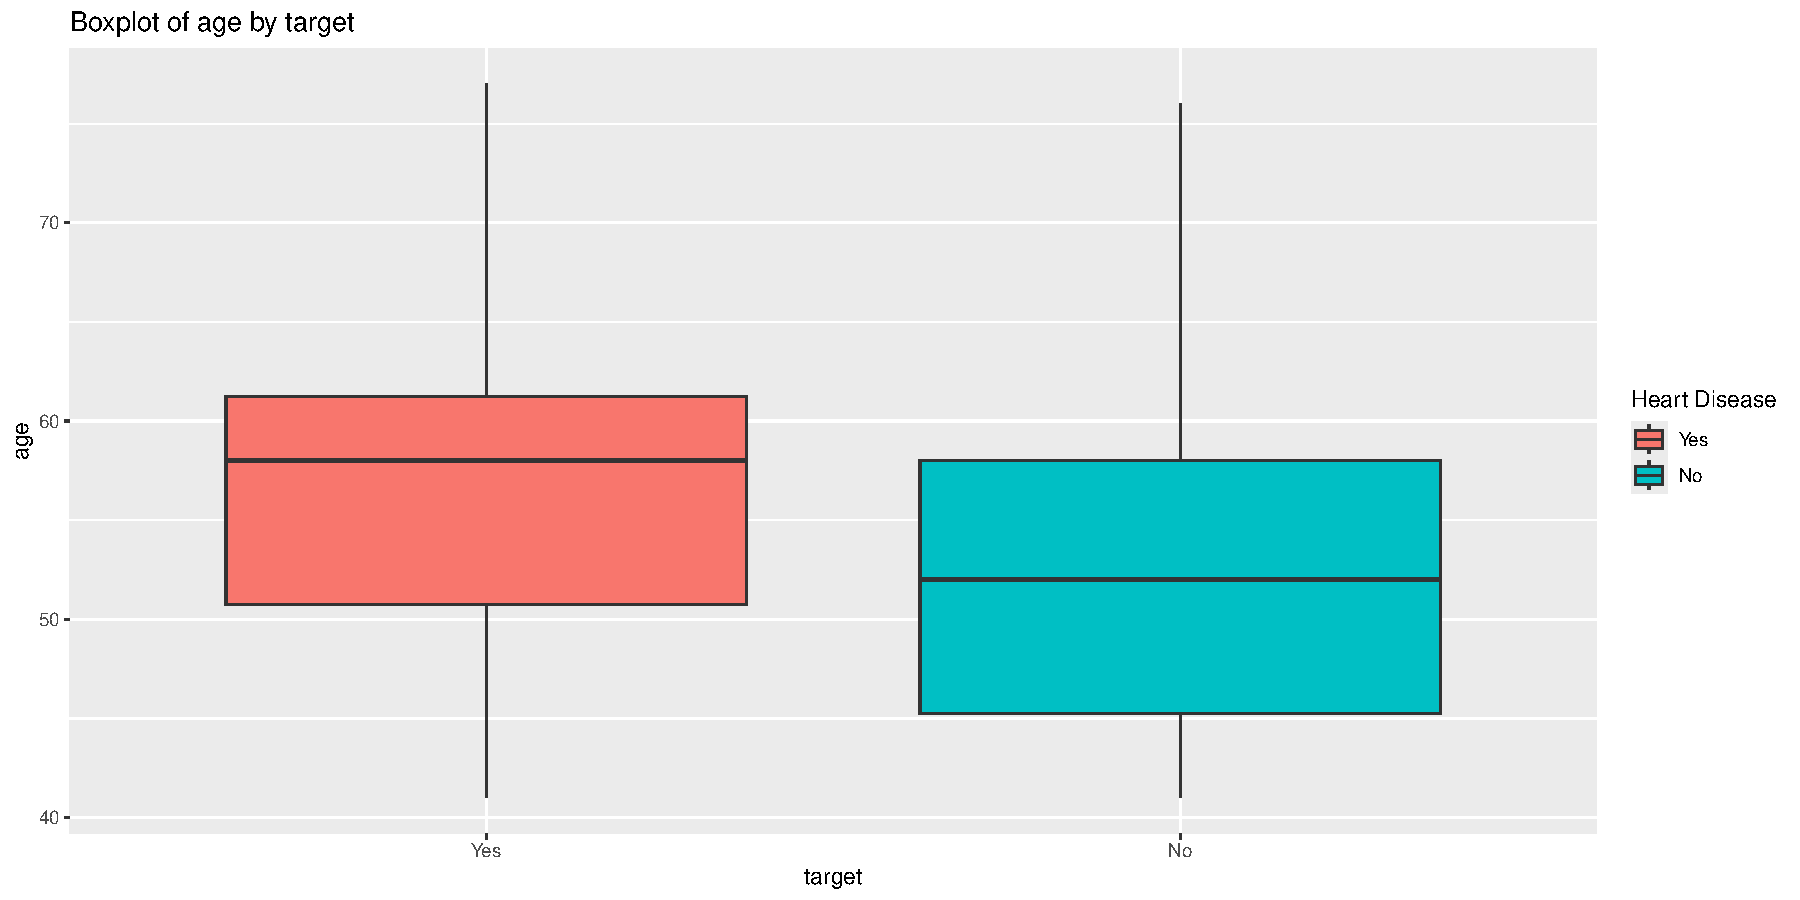
\includegraphics[keepaspectratio]{heart_disease_risks_files/figure-latex/unnamed-chunk-18-1.pdf}}

\textbf{Boxplot of Resting Blood Pressure (trestbps) by Heart Disease}

\begin{Shaded}
\begin{Highlighting}[]
\FunctionTok{HeartDiseaseBoxplot}\NormalTok{(}\StringTok{"target"}\NormalTok{, }\StringTok{"trestbps"}\NormalTok{)}
\end{Highlighting}
\end{Shaded}

\pandocbounded{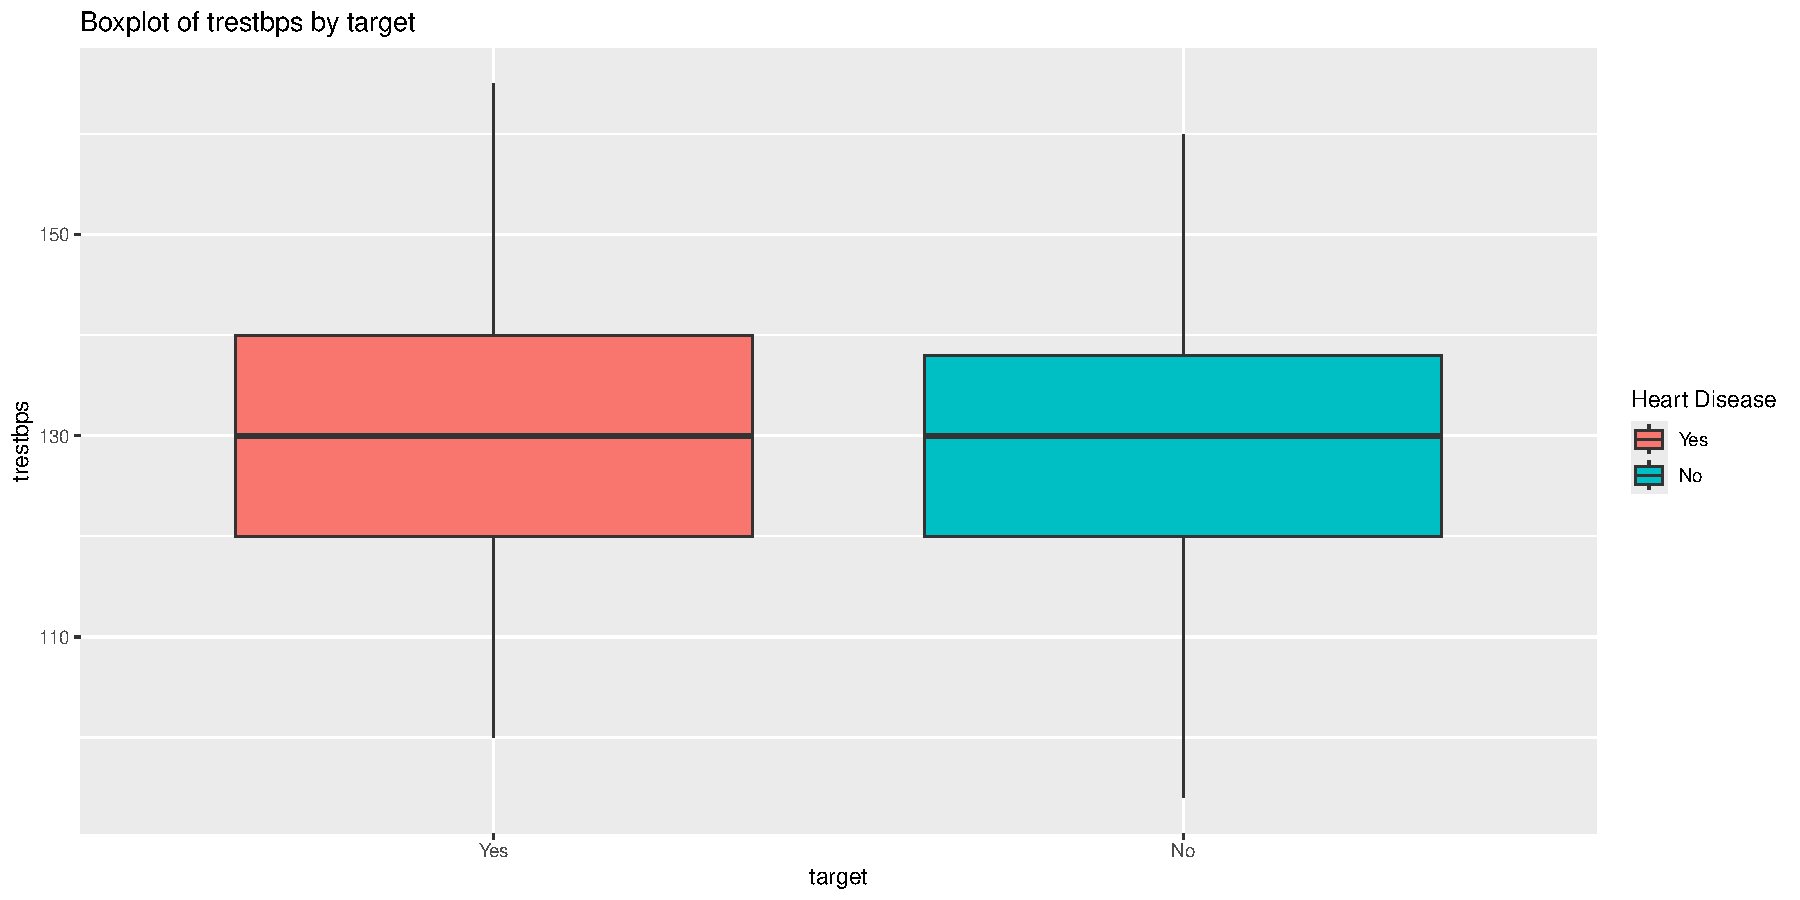
\includegraphics[keepaspectratio]{heart_disease_risks_files/figure-latex/unnamed-chunk-19-1.pdf}}

\textbf{Boxplot of Cholesterol (chol) by Heart Disease}

\begin{Shaded}
\begin{Highlighting}[]
\FunctionTok{HeartDiseaseBoxplot}\NormalTok{(}\StringTok{"target"}\NormalTok{, }\StringTok{"chol"}\NormalTok{)}
\end{Highlighting}
\end{Shaded}

\pandocbounded{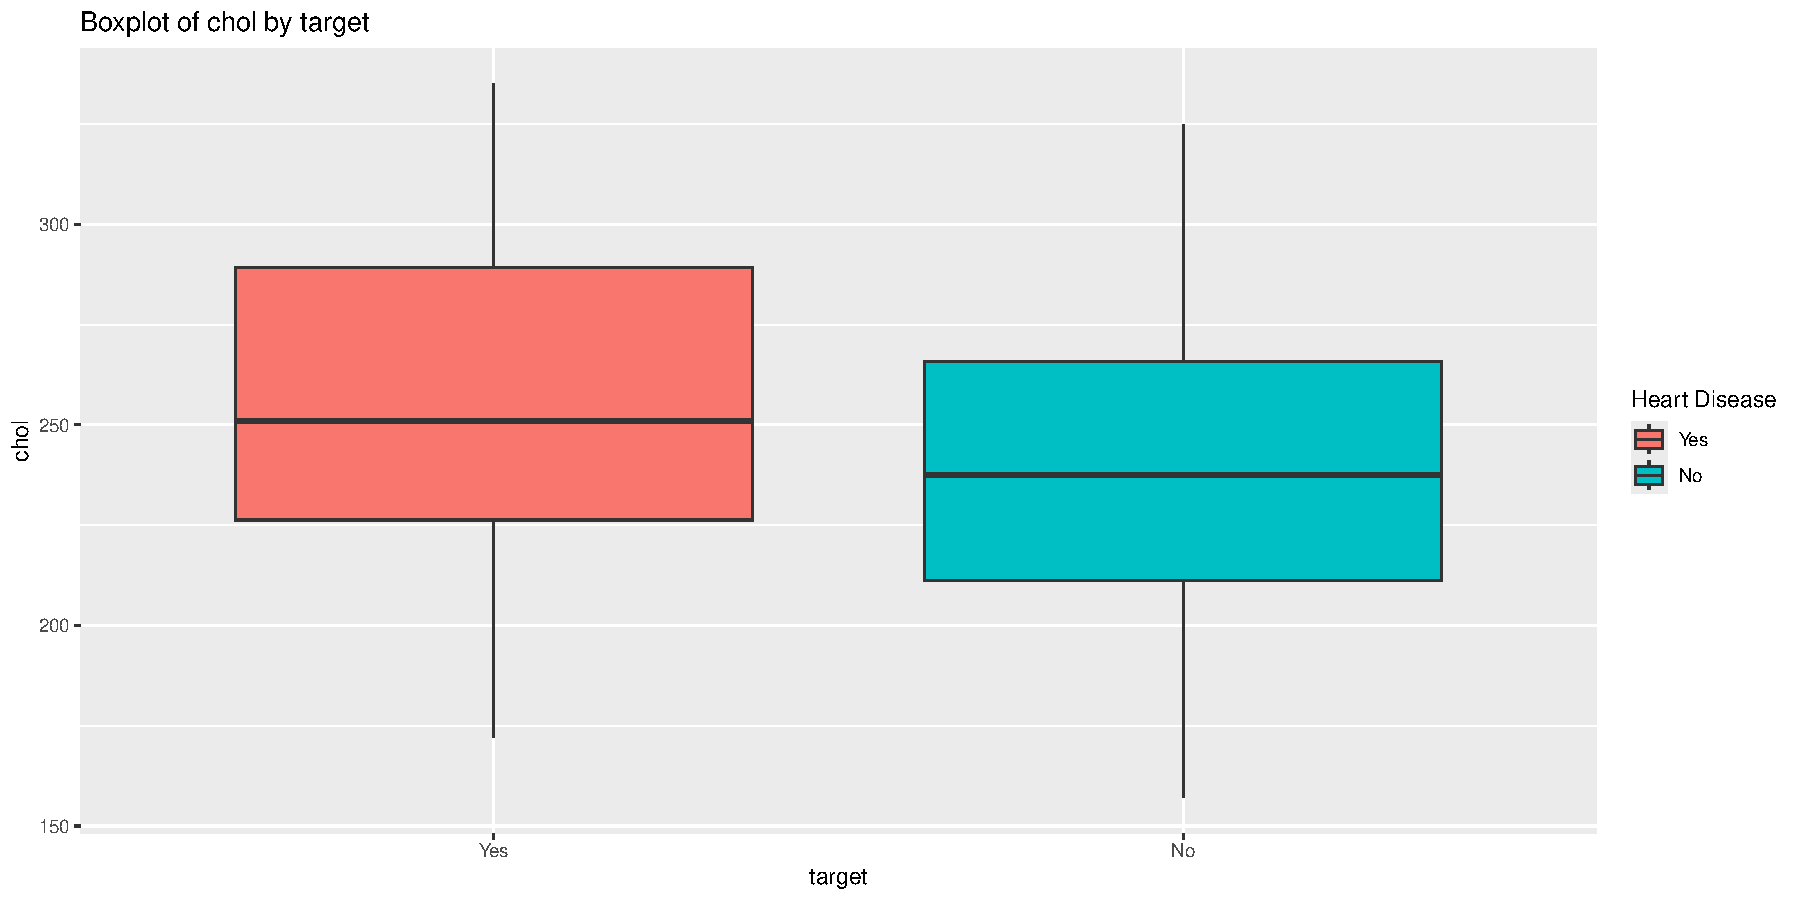
\includegraphics[keepaspectratio]{heart_disease_risks_files/figure-latex/unnamed-chunk-20-1.pdf}}

\textbf{Boxplot of Maximum Heart Rate Achieved (thalach) by Heart
Disease}

\begin{Shaded}
\begin{Highlighting}[]
\FunctionTok{HeartDiseaseBoxplot}\NormalTok{(}\StringTok{"target"}\NormalTok{, }\StringTok{"thalach"}\NormalTok{)}
\end{Highlighting}
\end{Shaded}

\pandocbounded{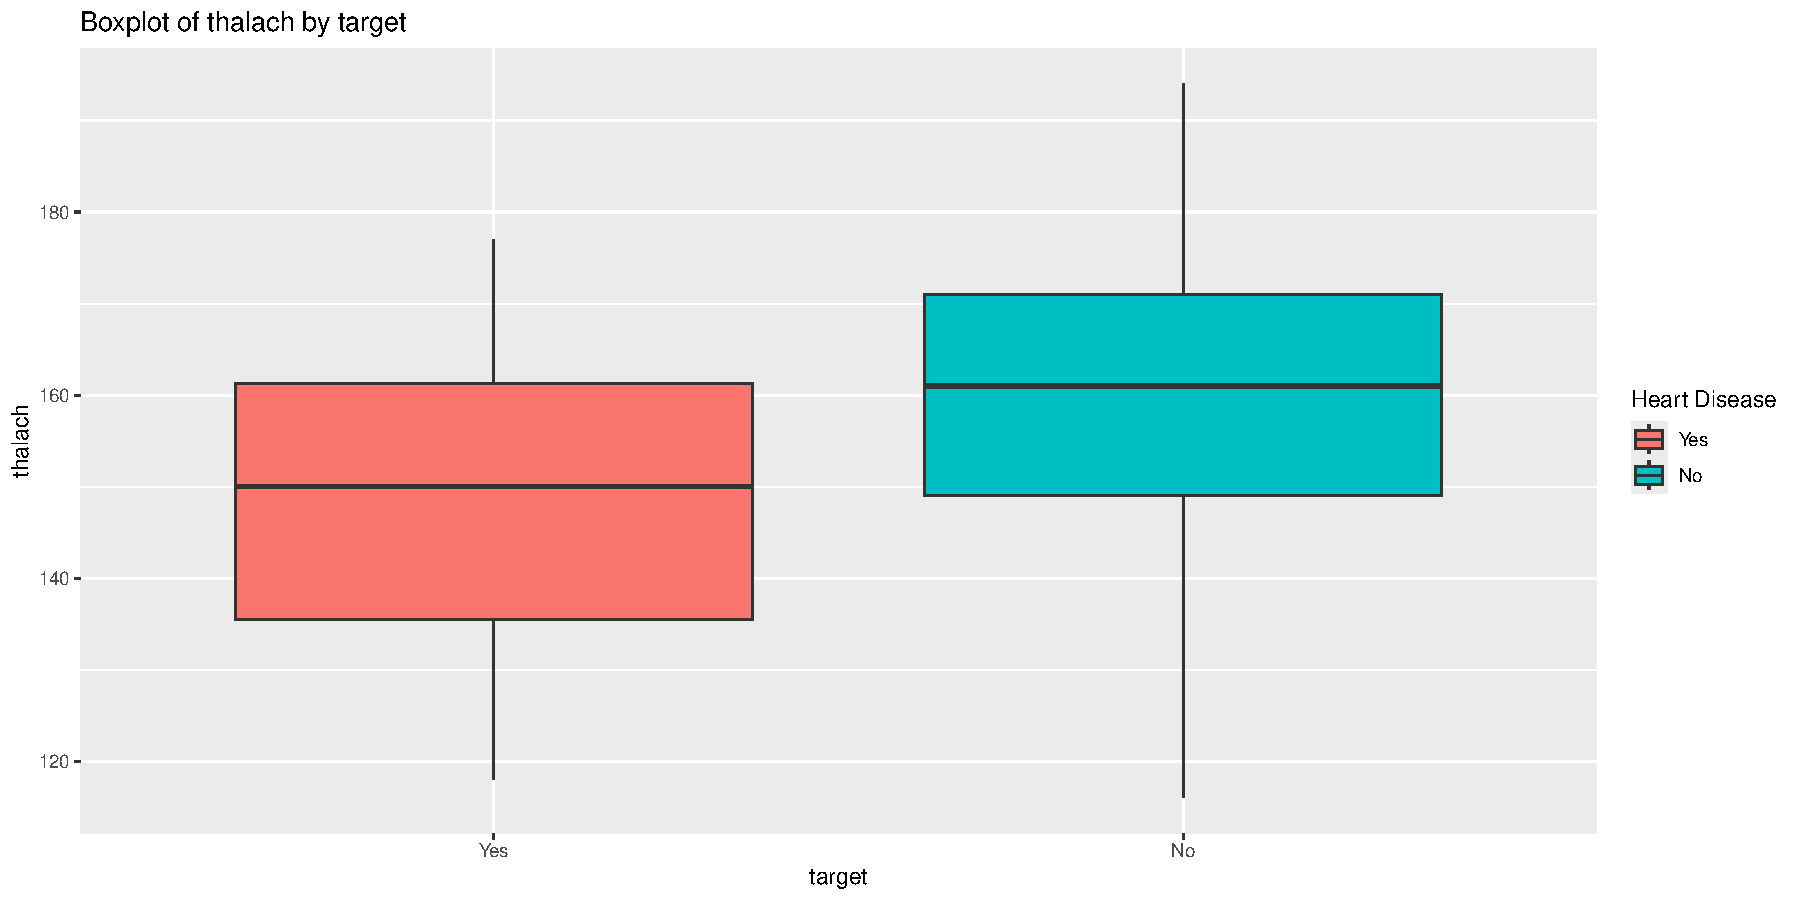
\includegraphics[keepaspectratio]{heart_disease_risks_files/figure-latex/unnamed-chunk-21-1.pdf}}

\textbf{Boxplot of ST Depression (oldpeak) by Heart Disease}

\begin{Shaded}
\begin{Highlighting}[]
\FunctionTok{HeartDiseaseBoxplot}\NormalTok{(}\StringTok{"target"}\NormalTok{, }\StringTok{"oldpeak"}\NormalTok{)}
\end{Highlighting}
\end{Shaded}

\pandocbounded{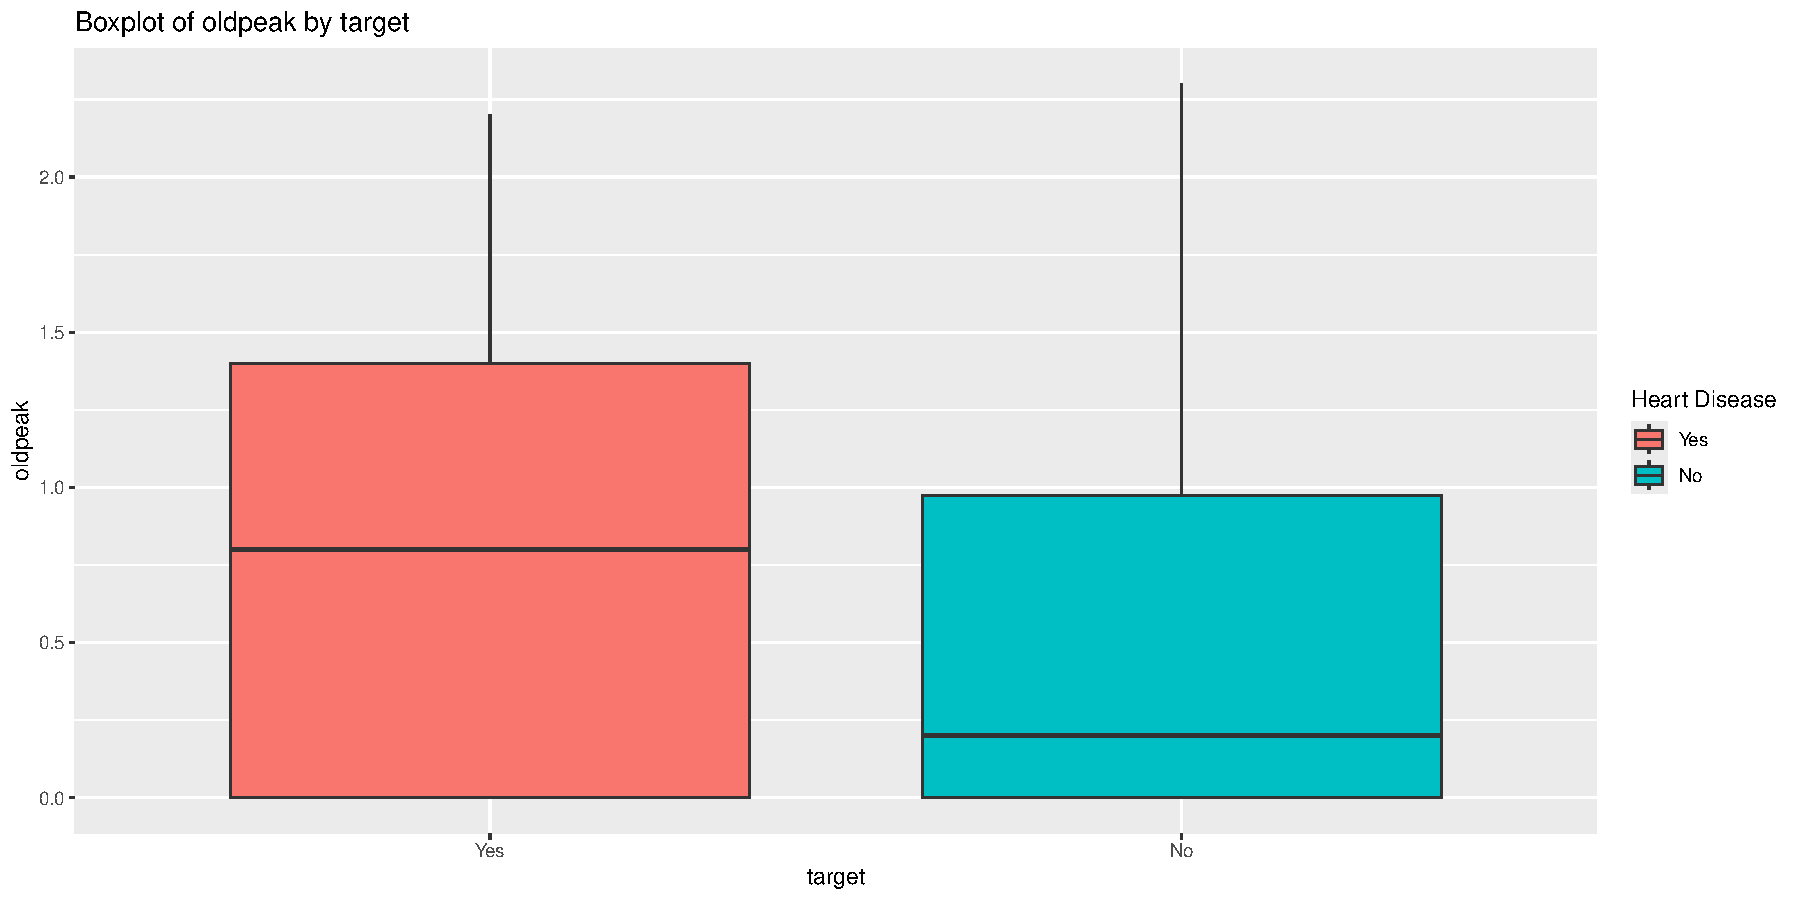
\includegraphics[keepaspectratio]{heart_disease_risks_files/figure-latex/unnamed-chunk-22-1.pdf}}

\textbf{Overall boxplots observations:}

\subsubsection{Barplots for categorical
variables}\label{barplots-for-categorical-variables}

\textbf{Heart disease distribution}

\begin{Shaded}
\begin{Highlighting}[]
\FunctionTok{ggplot}\NormalTok{(Heart.df, }\FunctionTok{aes}\NormalTok{(}\AttributeTok{x=}\NormalTok{target, }\AttributeTok{fill=}\NormalTok{target))}\SpecialCharTok{+}
  \FunctionTok{geom\_bar}\NormalTok{() }\SpecialCharTok{+}
  \FunctionTok{ggtitle}\NormalTok{(}\StringTok{"Distribution of Heart Disease"}\NormalTok{) }\SpecialCharTok{+}
  \FunctionTok{labs}\NormalTok{(}\AttributeTok{x =} \StringTok{"Heart Disease"}\NormalTok{, }\AttributeTok{fill =} \StringTok{"Heart Disease"}\NormalTok{)}
\end{Highlighting}
\end{Shaded}

\pandocbounded{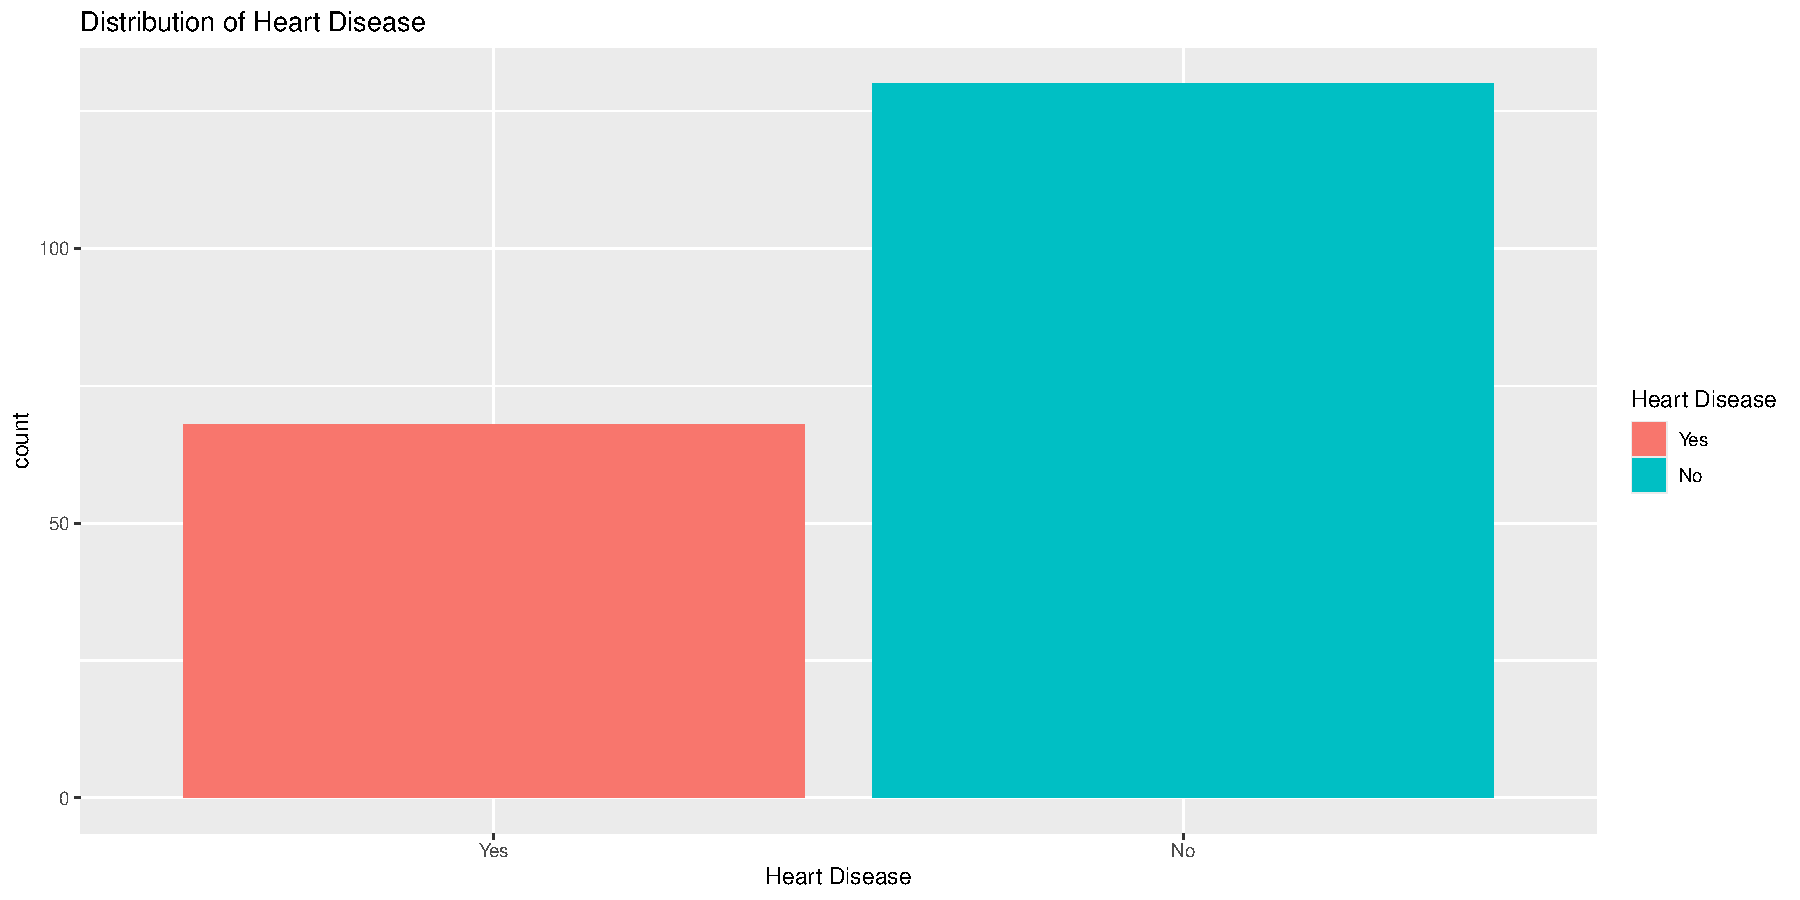
\includegraphics[keepaspectratio]{heart_disease_risks_files/figure-latex/unnamed-chunk-23-1.pdf}}

Visualize distribution of categorical variables by heart disease
presence.

\begin{Shaded}
\begin{Highlighting}[]
\FunctionTok{HeartDiseaseBar}\NormalTok{(}\StringTok{"sex"}\NormalTok{)}
\end{Highlighting}
\end{Shaded}

\pandocbounded{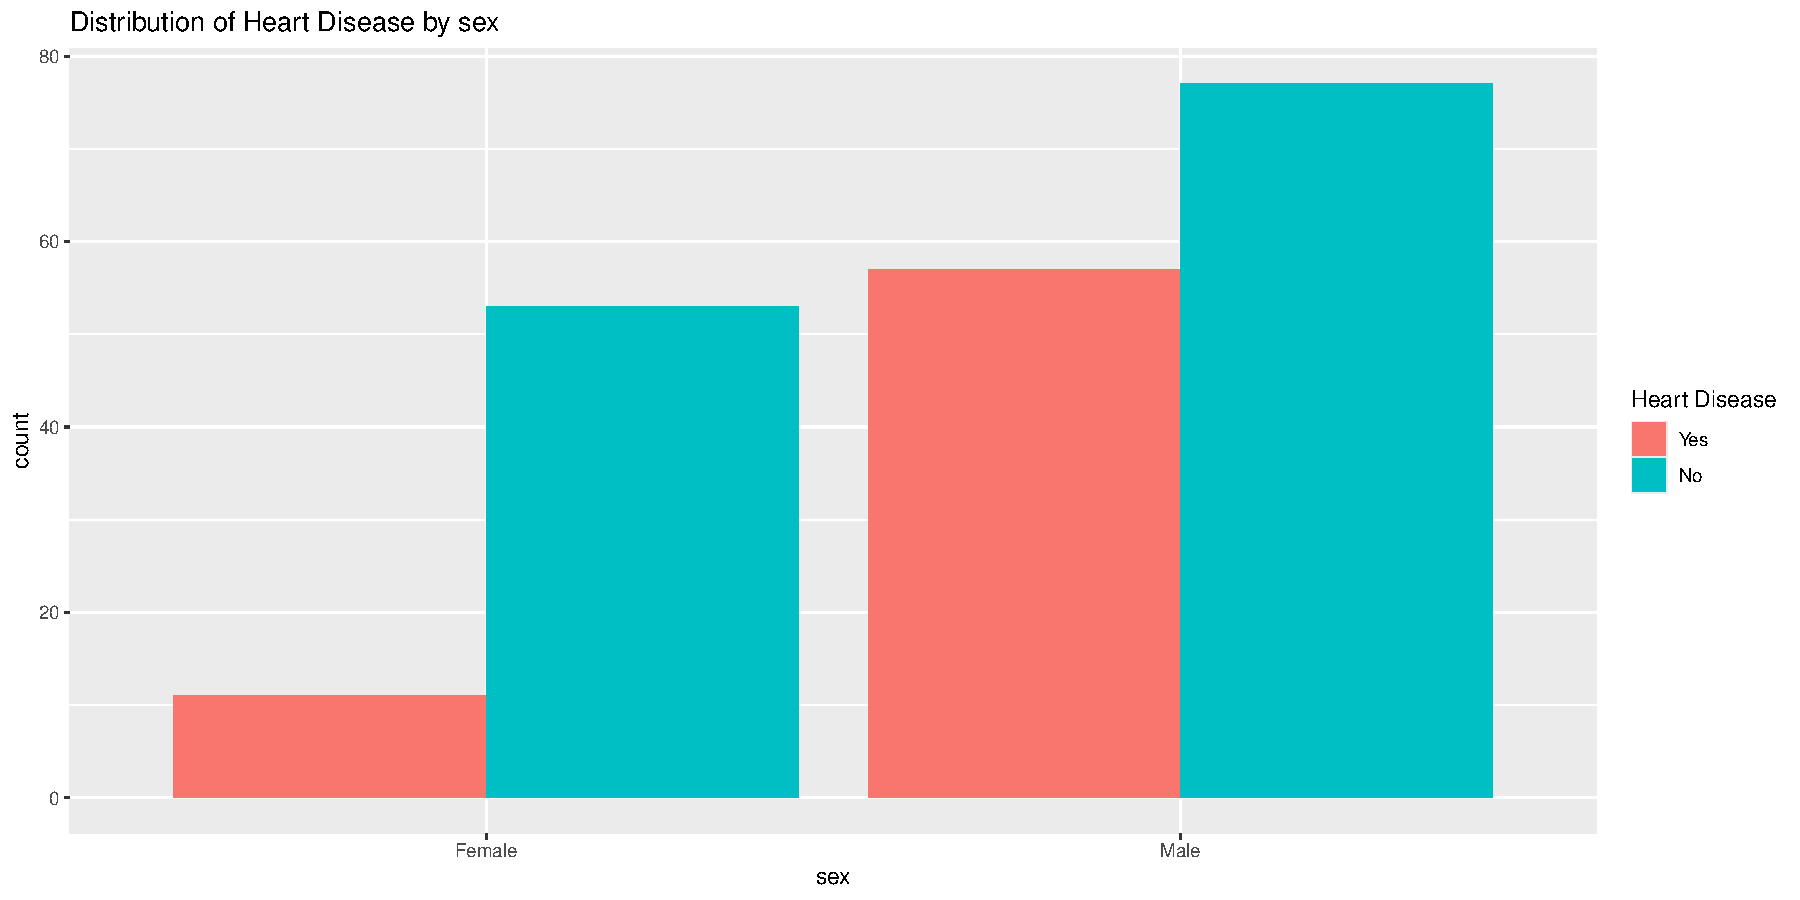
\includegraphics[keepaspectratio]{heart_disease_risks_files/figure-latex/unnamed-chunk-24-1.pdf}}

\begin{Shaded}
\begin{Highlighting}[]
\FunctionTok{HeartDiseaseBar}\NormalTok{(}\StringTok{"cp"}\NormalTok{)}
\end{Highlighting}
\end{Shaded}

\pandocbounded{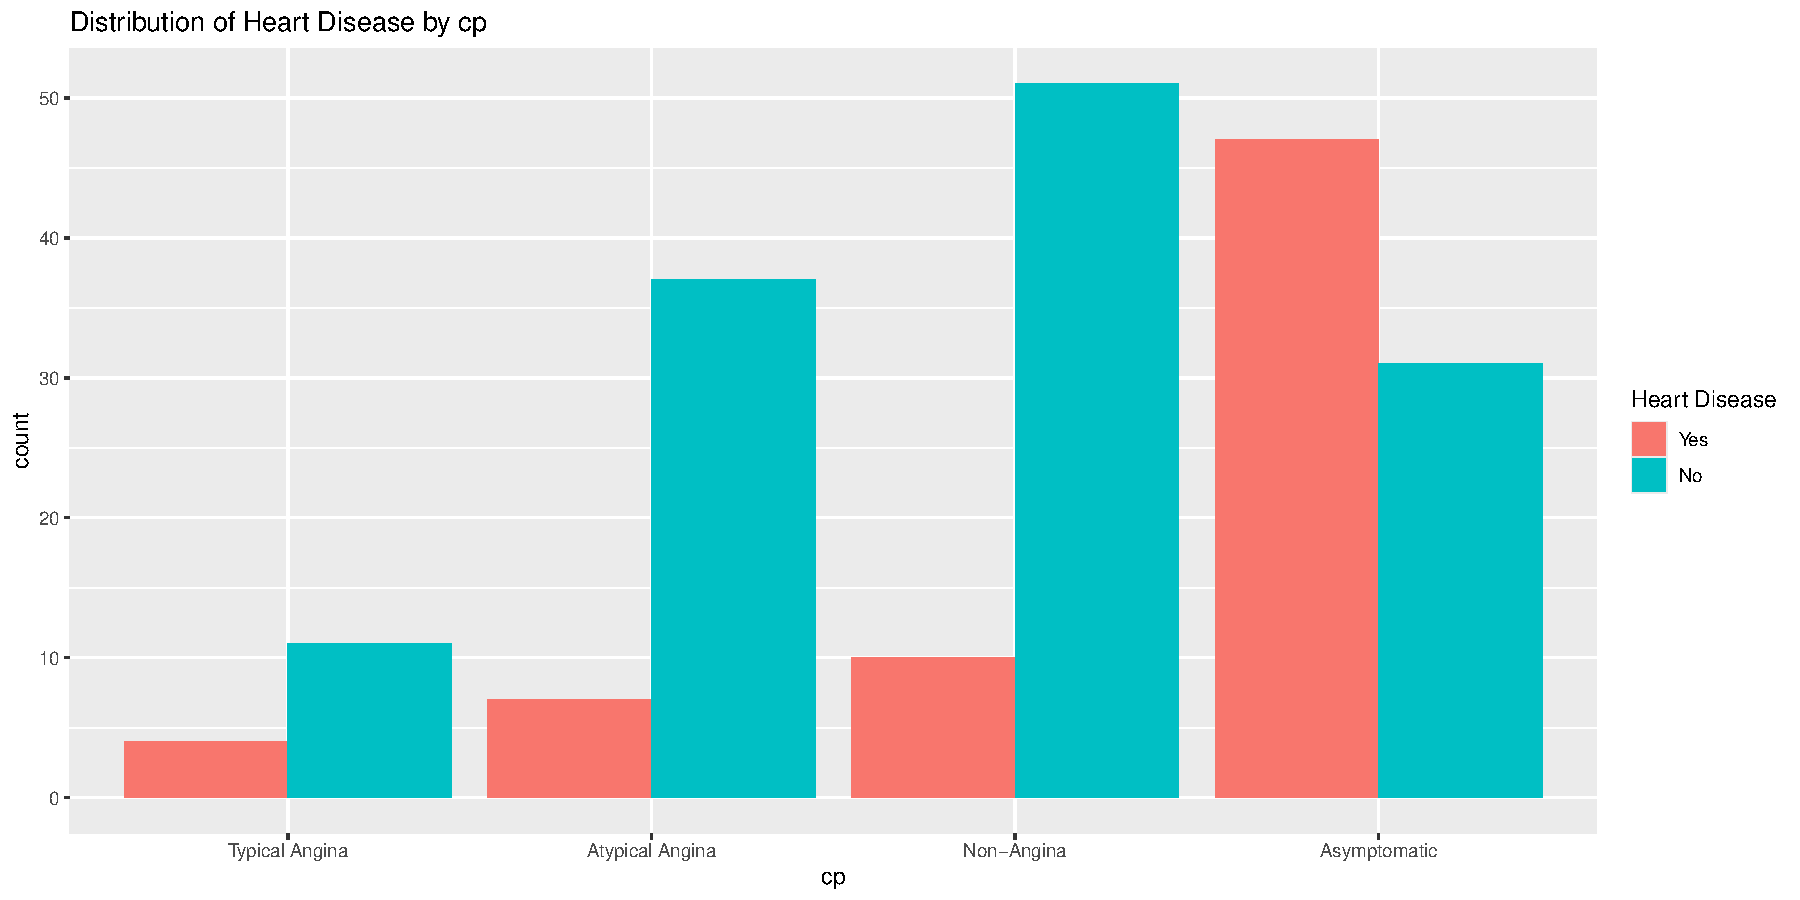
\includegraphics[keepaspectratio]{heart_disease_risks_files/figure-latex/unnamed-chunk-24-2.pdf}}

\begin{Shaded}
\begin{Highlighting}[]
\FunctionTok{HeartDiseaseBar}\NormalTok{(}\StringTok{"fbs"}\NormalTok{)}
\end{Highlighting}
\end{Shaded}

\pandocbounded{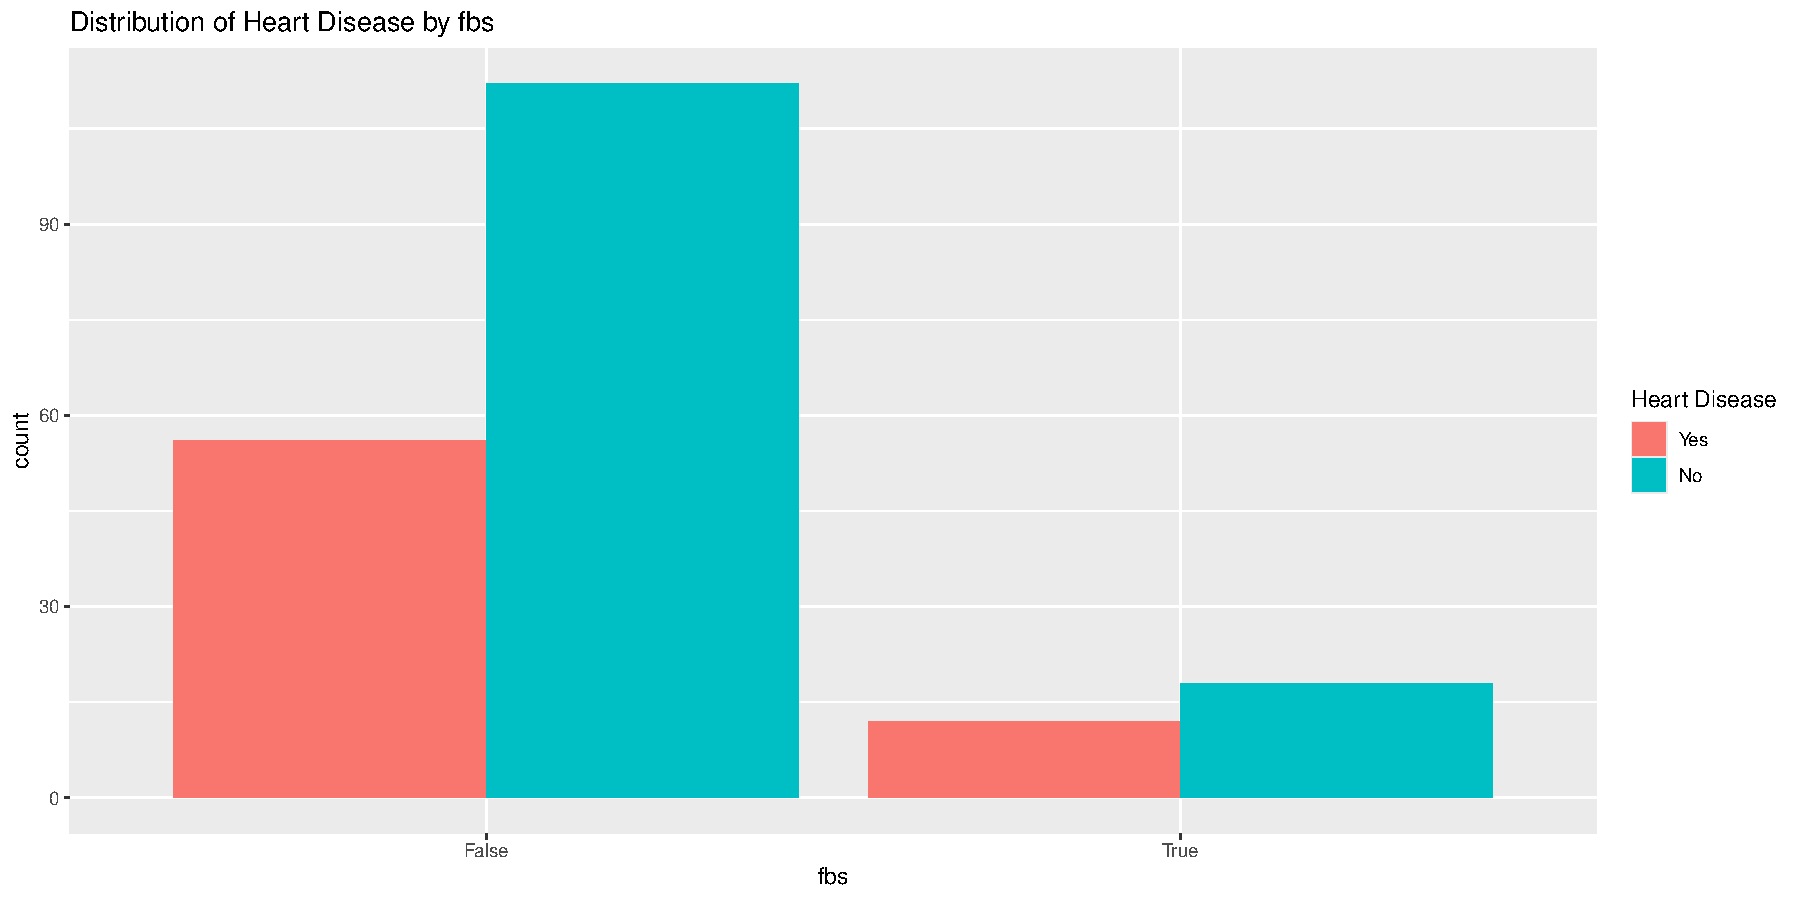
\includegraphics[keepaspectratio]{heart_disease_risks_files/figure-latex/unnamed-chunk-24-3.pdf}}

\begin{Shaded}
\begin{Highlighting}[]
\FunctionTok{HeartDiseaseBar}\NormalTok{(}\StringTok{"restecg"}\NormalTok{)}
\end{Highlighting}
\end{Shaded}

\pandocbounded{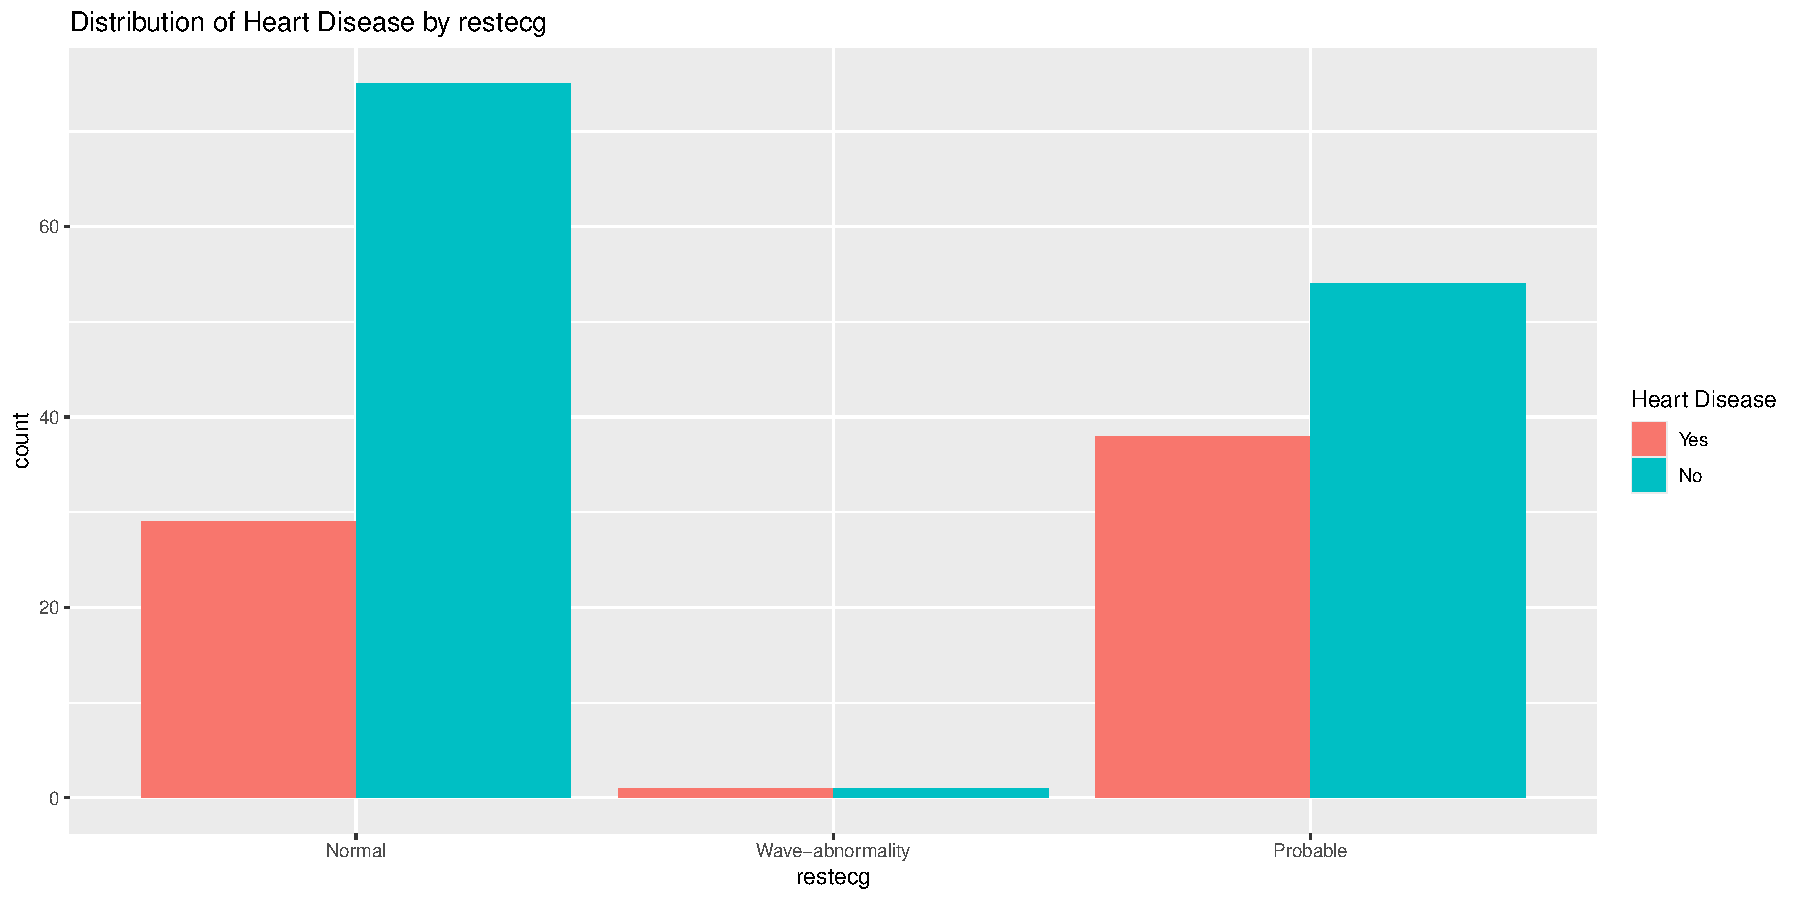
\includegraphics[keepaspectratio]{heart_disease_risks_files/figure-latex/unnamed-chunk-24-4.pdf}}

\begin{Shaded}
\begin{Highlighting}[]
\FunctionTok{HeartDiseaseBar}\NormalTok{(}\StringTok{"exang"}\NormalTok{)}
\end{Highlighting}
\end{Shaded}

\pandocbounded{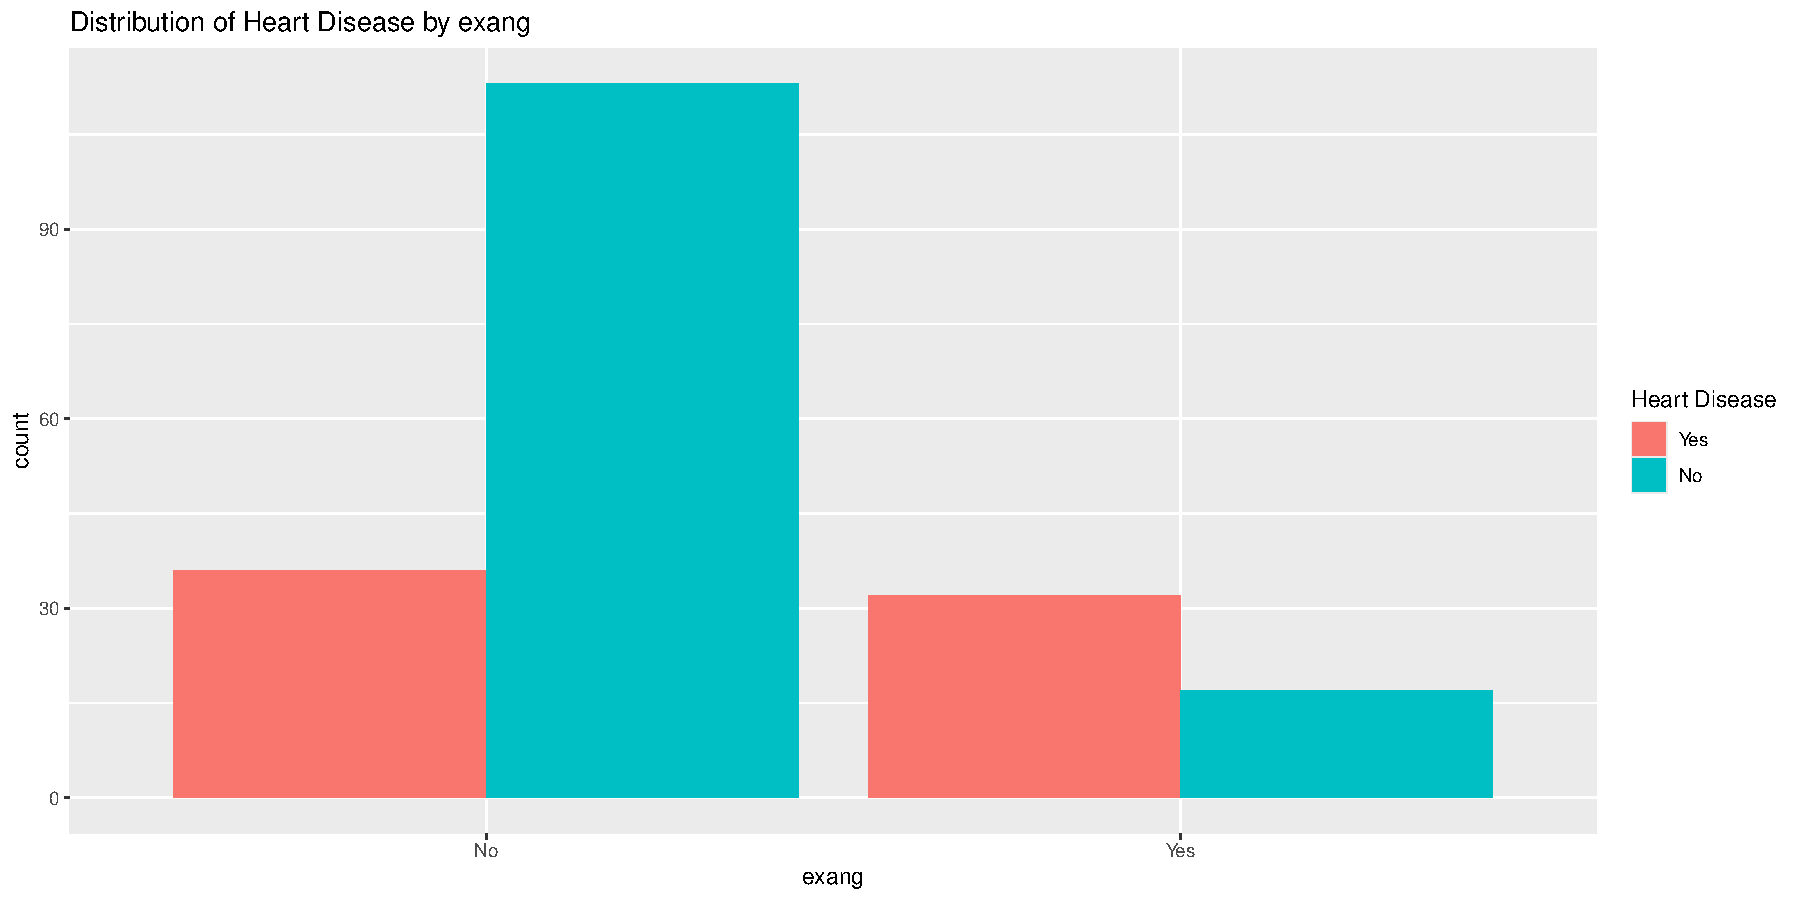
\includegraphics[keepaspectratio]{heart_disease_risks_files/figure-latex/unnamed-chunk-24-5.pdf}}

\begin{Shaded}
\begin{Highlighting}[]
\FunctionTok{HeartDiseaseBar}\NormalTok{(}\StringTok{"slope"}\NormalTok{)}
\end{Highlighting}
\end{Shaded}

\pandocbounded{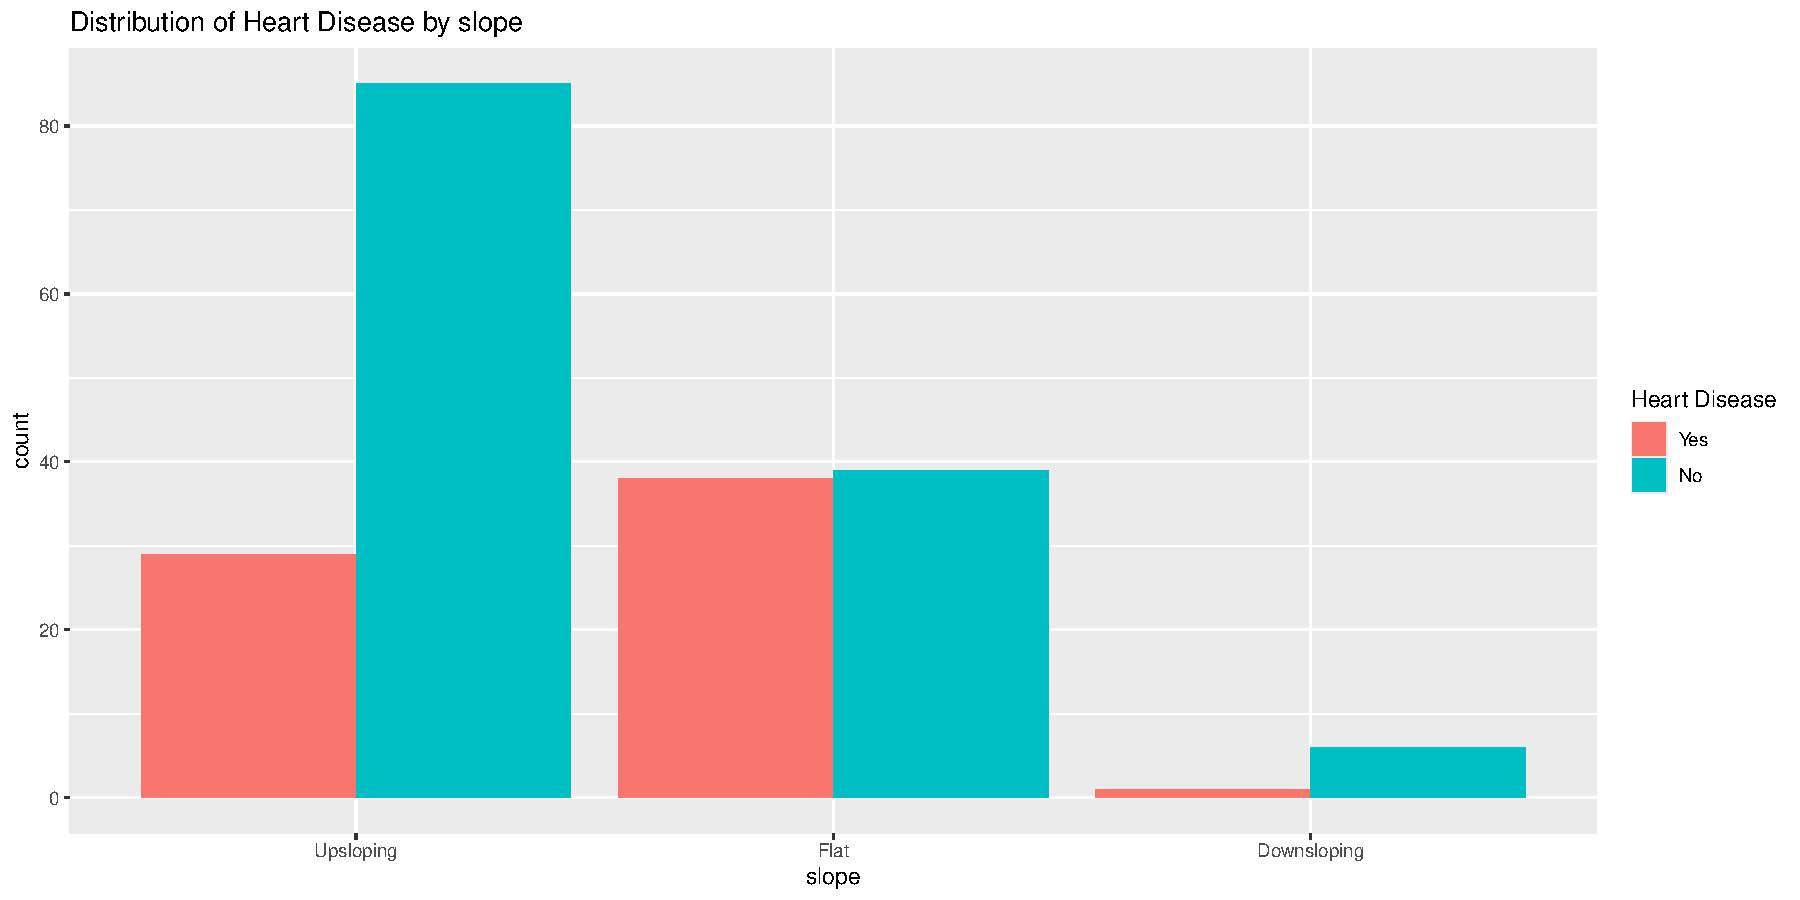
\includegraphics[keepaspectratio]{heart_disease_risks_files/figure-latex/unnamed-chunk-24-6.pdf}}

\begin{Shaded}
\begin{Highlighting}[]
\FunctionTok{HeartDiseaseBar}\NormalTok{(}\StringTok{"thal"}\NormalTok{)}
\end{Highlighting}
\end{Shaded}

\pandocbounded{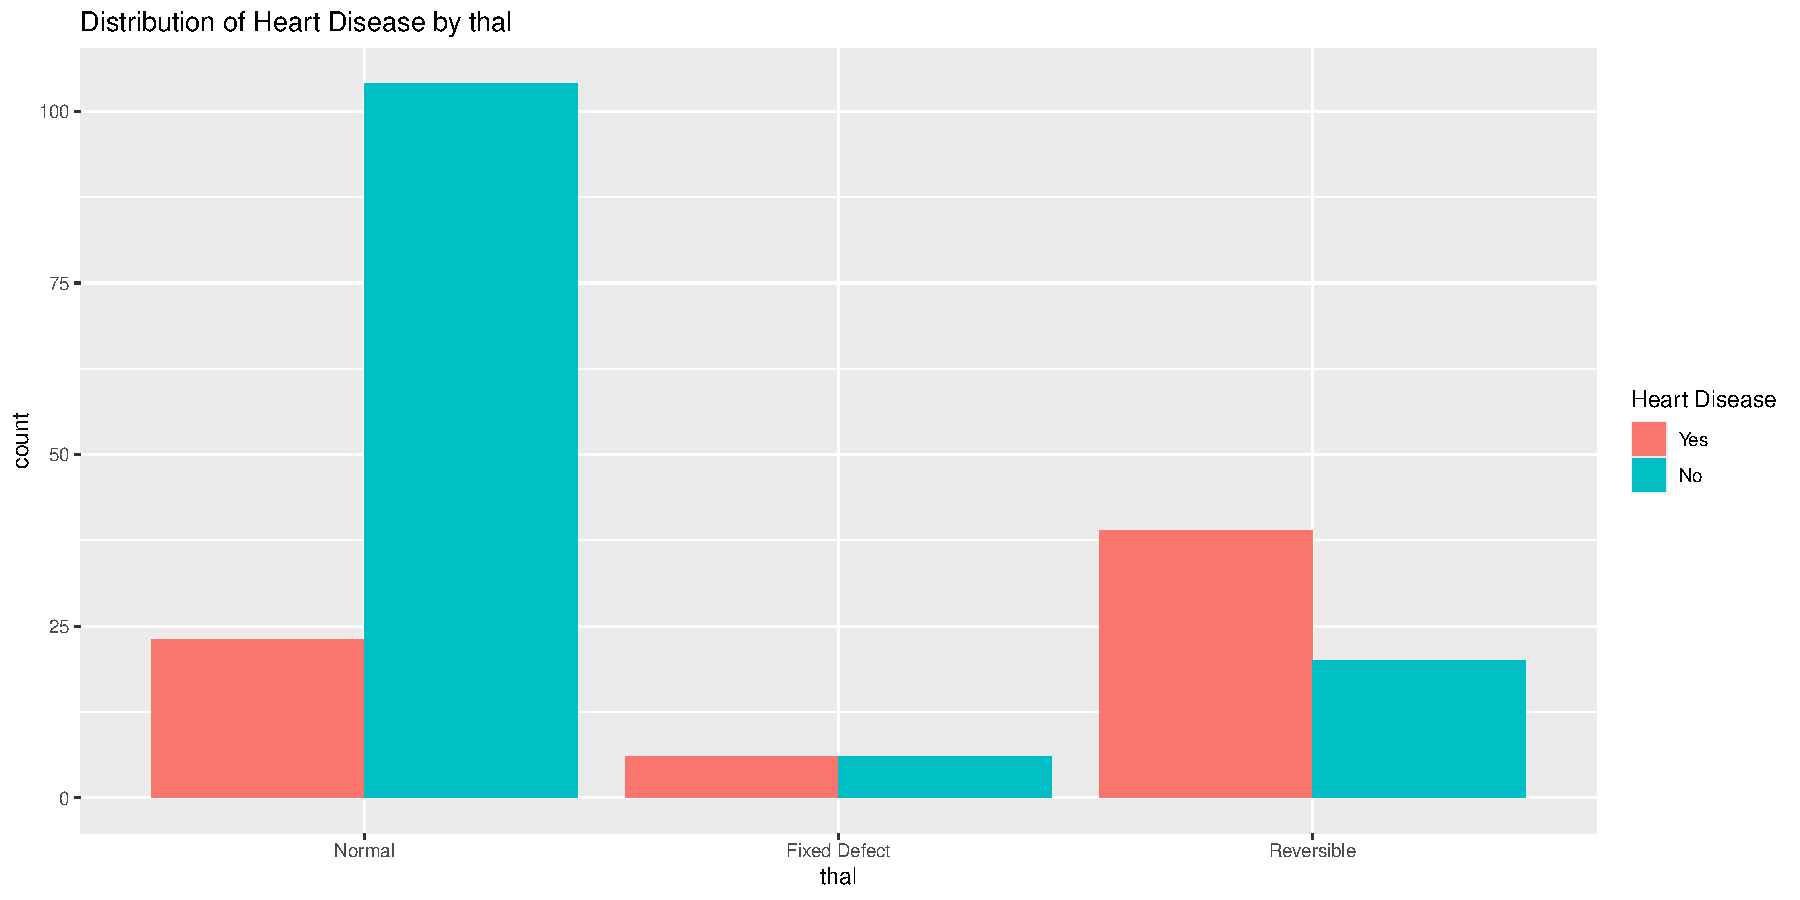
\includegraphics[keepaspectratio]{heart_disease_risks_files/figure-latex/unnamed-chunk-24-7.pdf}}

\subsubsection{Histograms for Numerical
Variables}\label{histograms-for-numerical-variables}

\begin{Shaded}
\begin{Highlighting}[]
\FunctionTok{HeartDiseaseHist}\NormalTok{(}\StringTok{"age"}\NormalTok{)}
\end{Highlighting}
\end{Shaded}

\pandocbounded{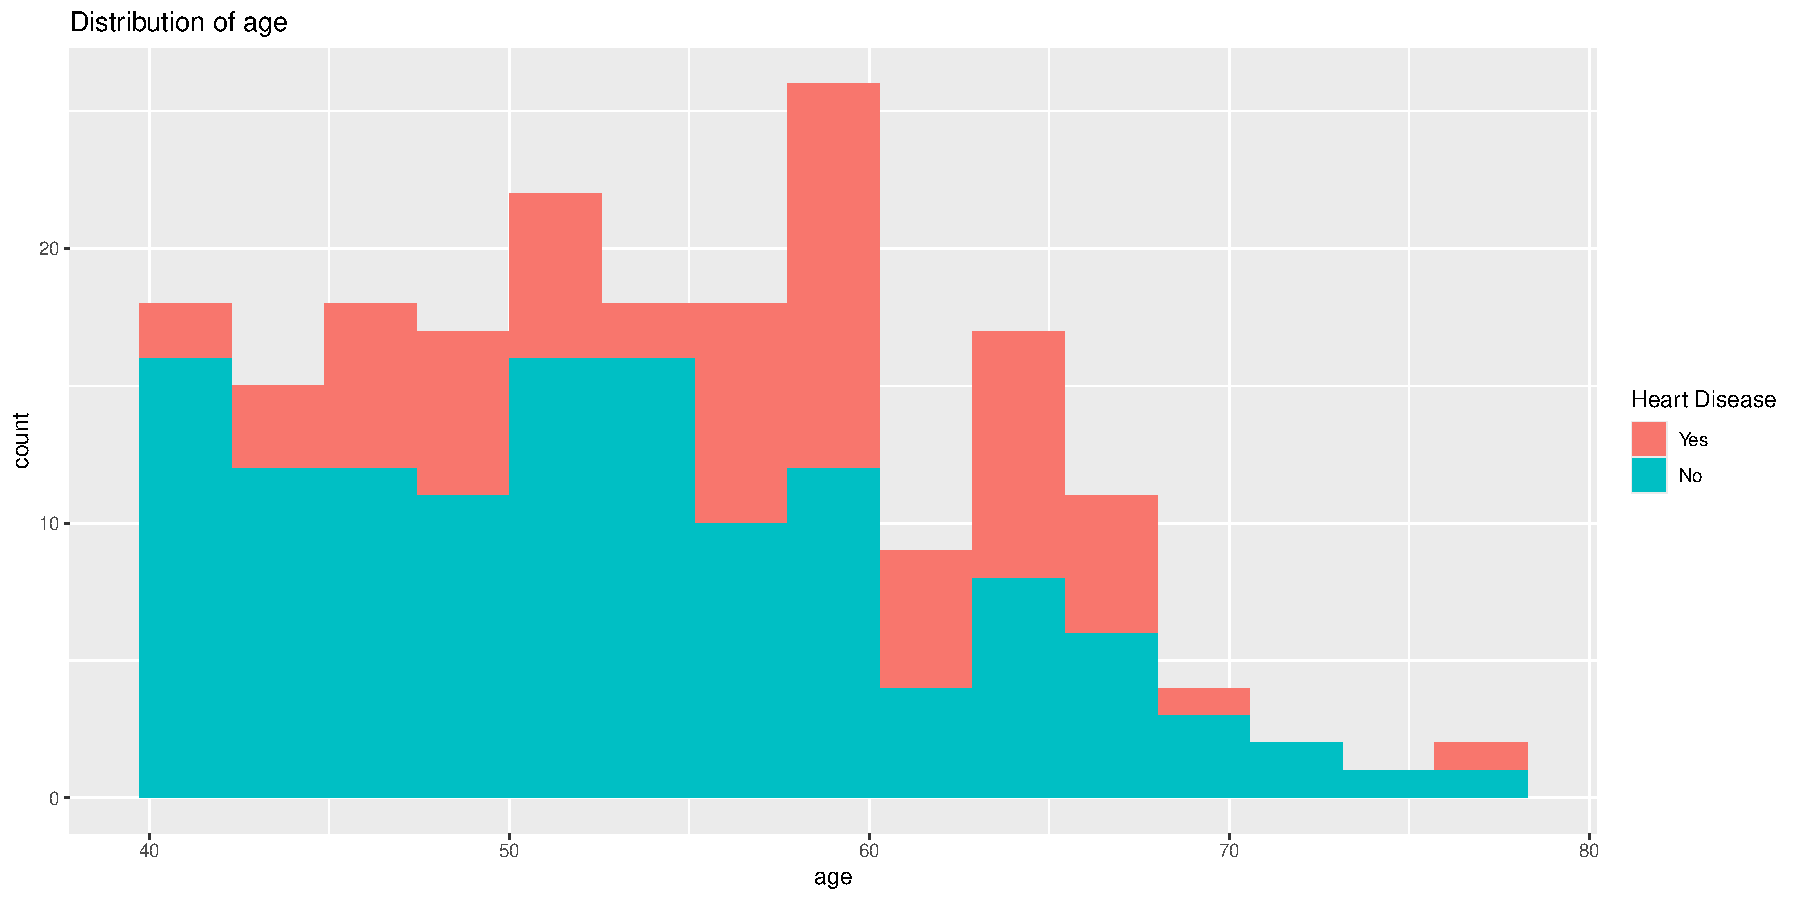
\includegraphics[keepaspectratio]{heart_disease_risks_files/figure-latex/unnamed-chunk-25-1.pdf}}

\begin{Shaded}
\begin{Highlighting}[]
\FunctionTok{HeartDiseaseHist}\NormalTok{(}\StringTok{"trestbps"}\NormalTok{)}
\end{Highlighting}
\end{Shaded}

\pandocbounded{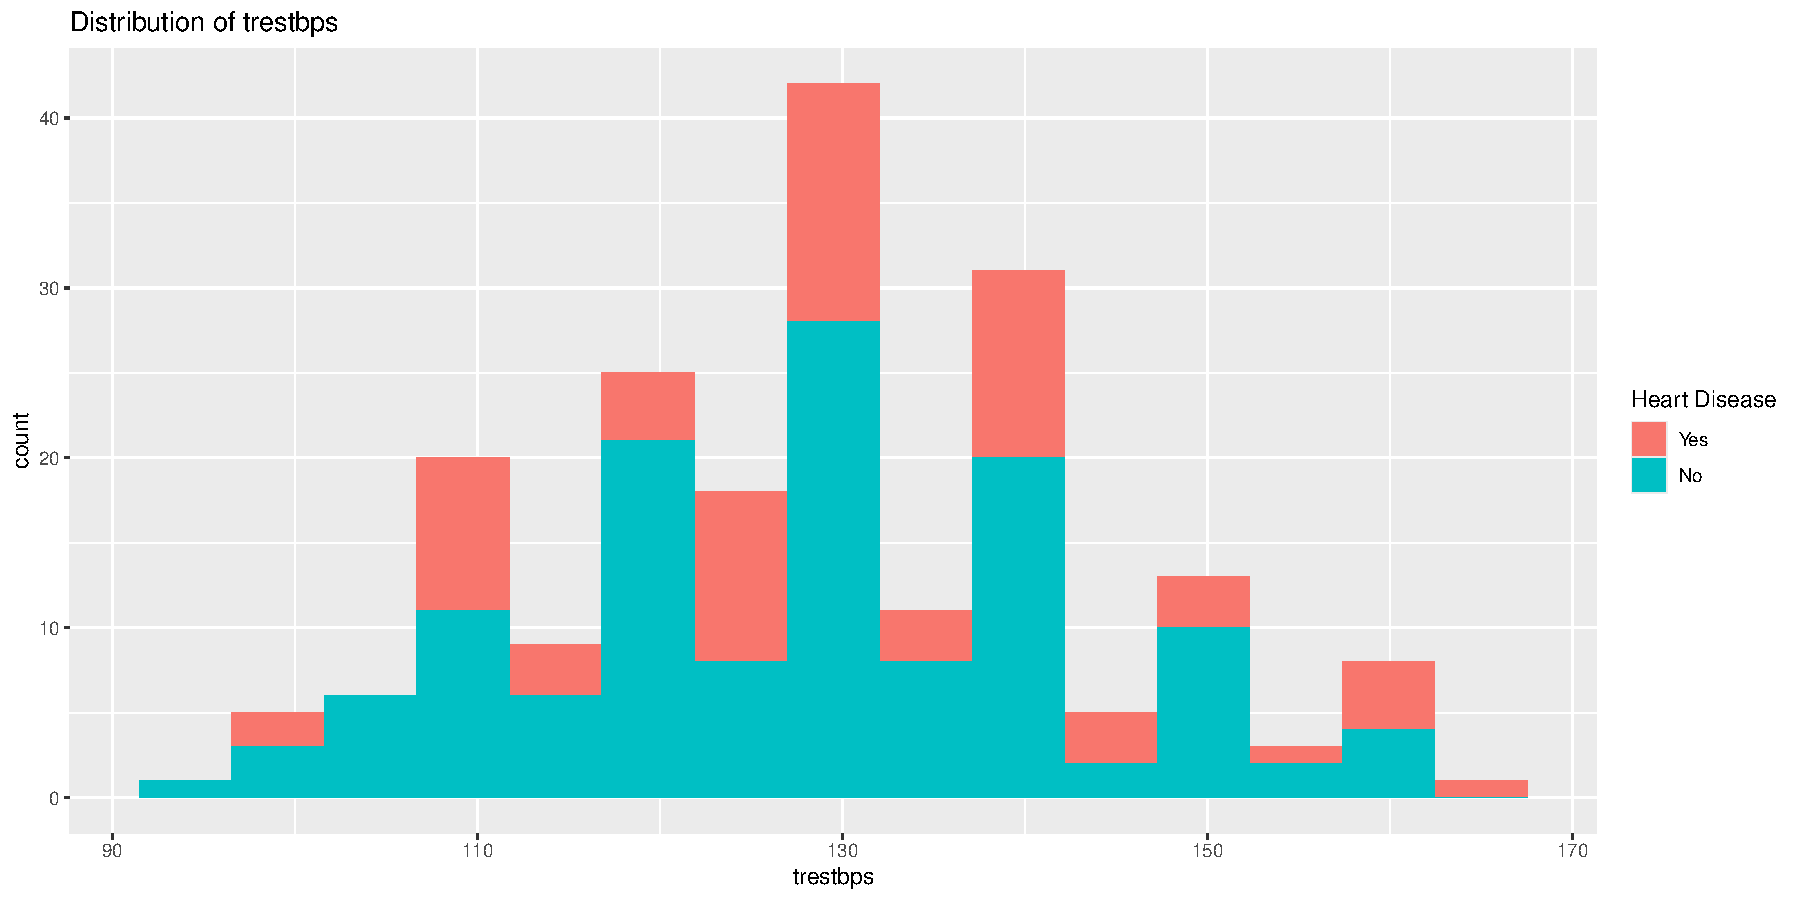
\includegraphics[keepaspectratio]{heart_disease_risks_files/figure-latex/unnamed-chunk-25-2.pdf}}

\begin{Shaded}
\begin{Highlighting}[]
\FunctionTok{HeartDiseaseHist}\NormalTok{(}\StringTok{"chol"}\NormalTok{)}
\end{Highlighting}
\end{Shaded}

\pandocbounded{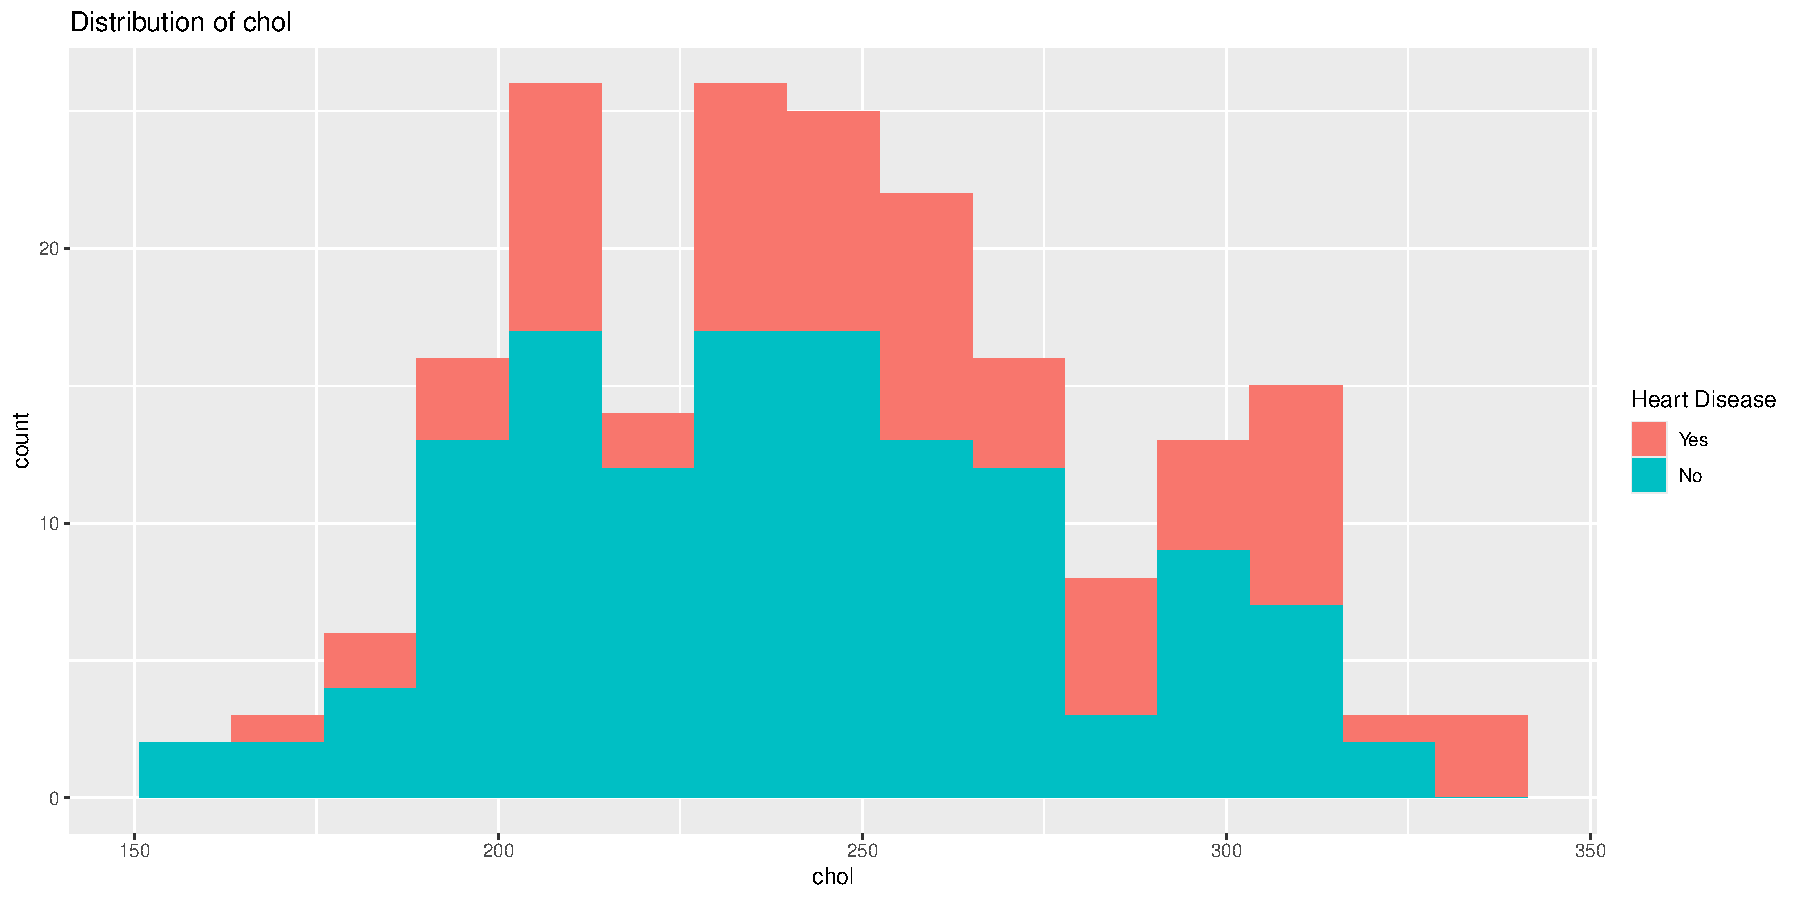
\includegraphics[keepaspectratio]{heart_disease_risks_files/figure-latex/unnamed-chunk-25-3.pdf}}

\begin{Shaded}
\begin{Highlighting}[]
\FunctionTok{HeartDiseaseHist}\NormalTok{(}\StringTok{"thalach"}\NormalTok{)}
\end{Highlighting}
\end{Shaded}

\pandocbounded{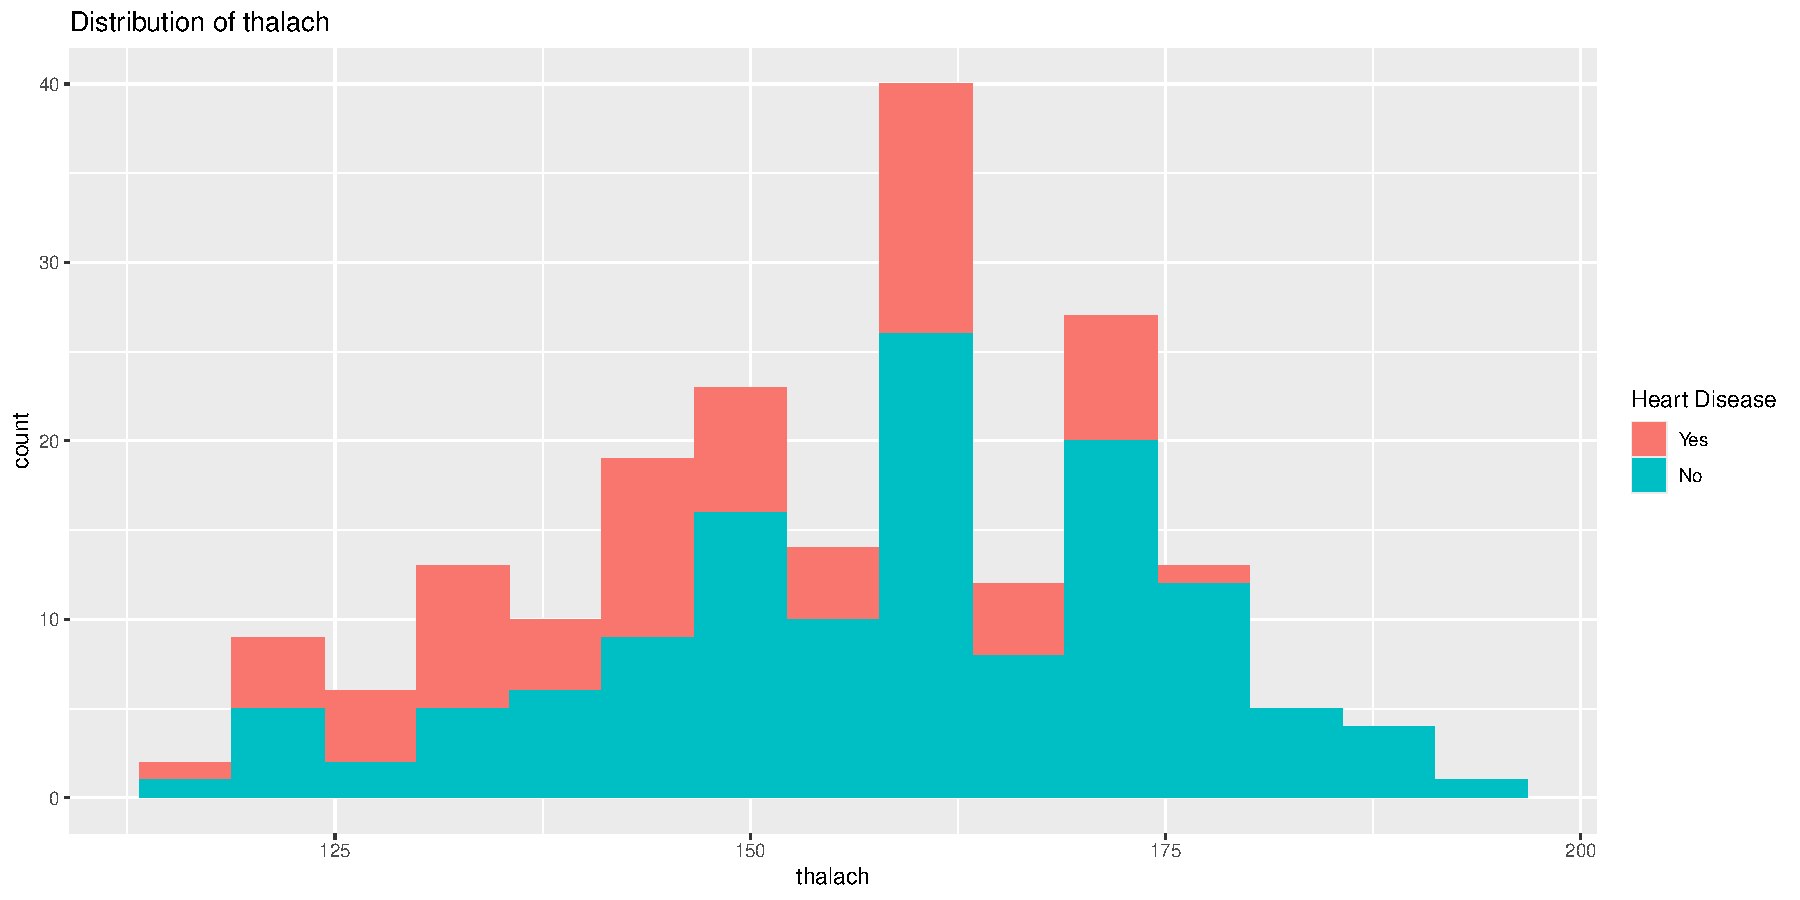
\includegraphics[keepaspectratio]{heart_disease_risks_files/figure-latex/unnamed-chunk-25-4.pdf}}

\begin{Shaded}
\begin{Highlighting}[]
\FunctionTok{HeartDiseaseHist}\NormalTok{(}\StringTok{"oldpeak"}\NormalTok{)}
\end{Highlighting}
\end{Shaded}

\pandocbounded{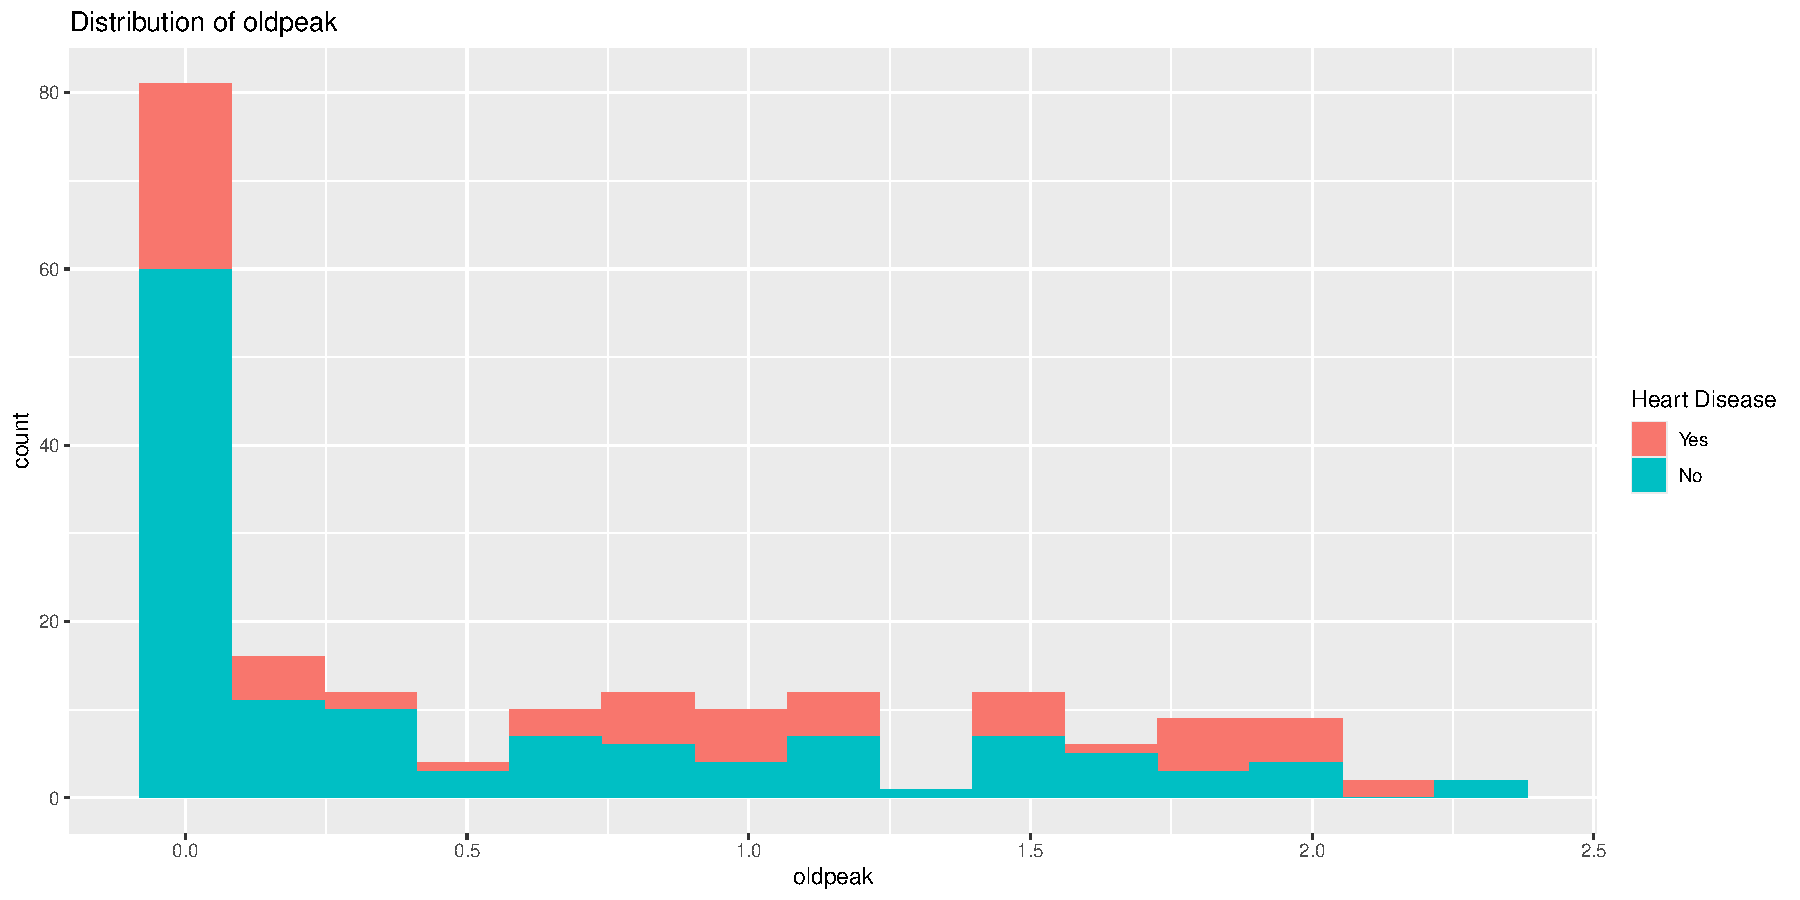
\includegraphics[keepaspectratio]{heart_disease_risks_files/figure-latex/unnamed-chunk-25-5.pdf}}

\subsubsection{Scatterplots for numerical
variables}\label{scatterplots-for-numerical-variables}

\begin{Shaded}
\begin{Highlighting}[]
\FunctionTok{HeartDiseaseScatter}\NormalTok{(}\StringTok{"age"}\NormalTok{, }\StringTok{"oldpeak"}\NormalTok{)}
\end{Highlighting}
\end{Shaded}

\pandocbounded{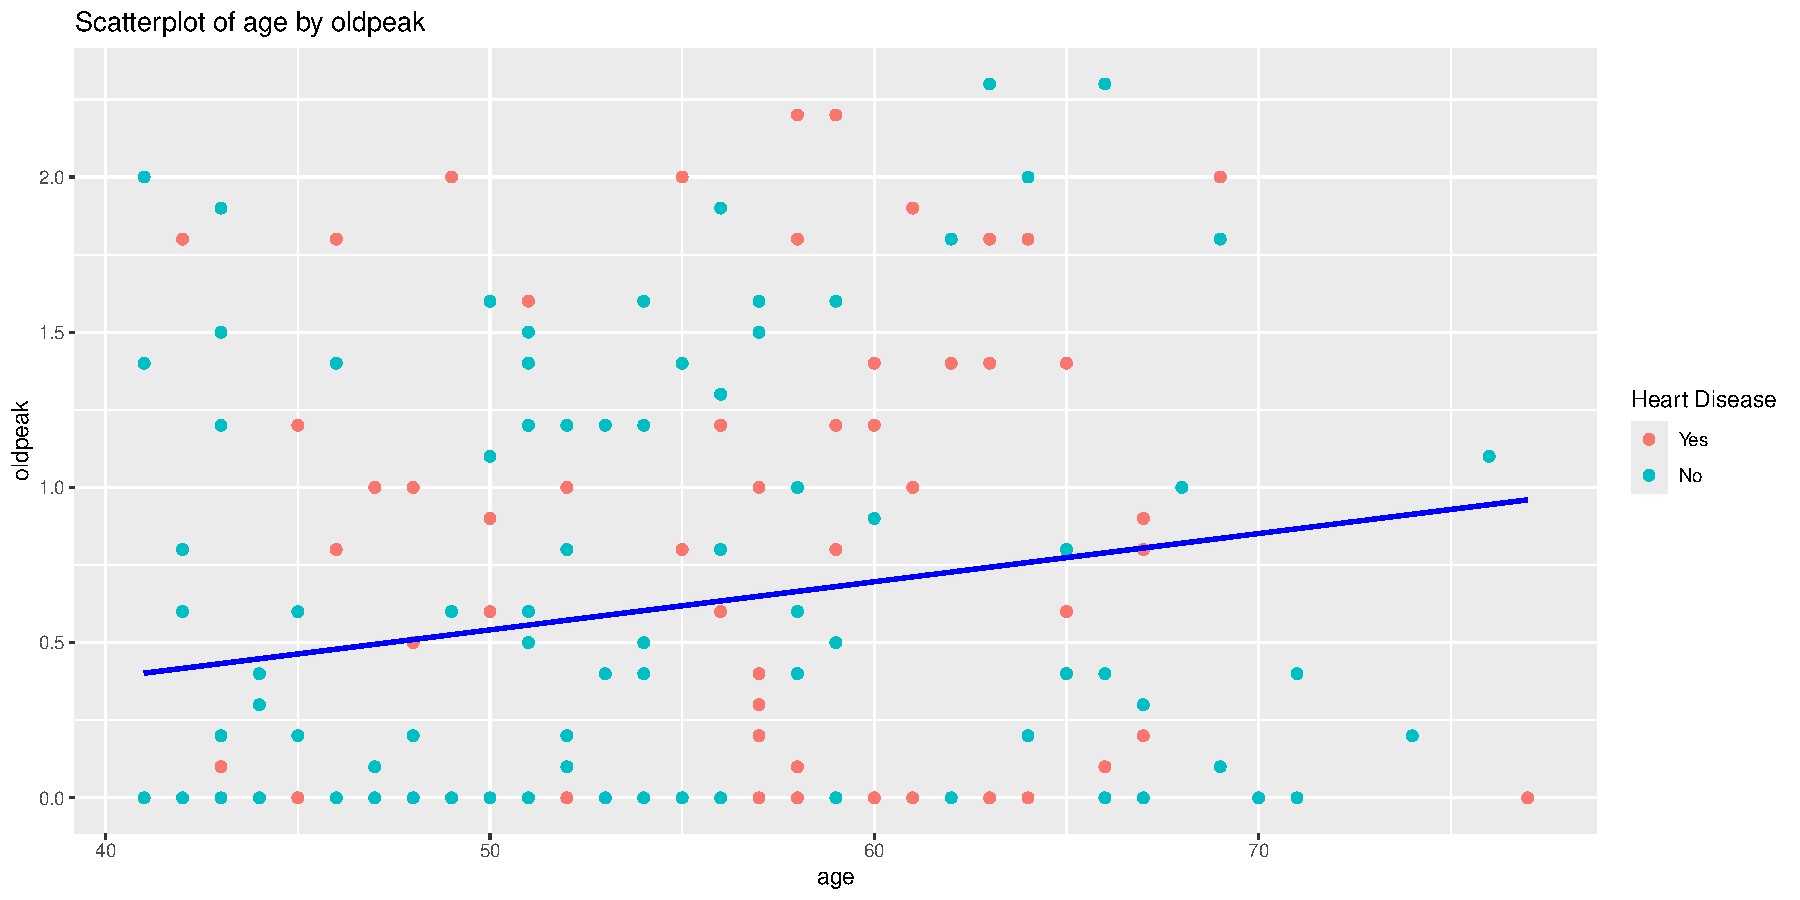
\includegraphics[keepaspectratio]{heart_disease_risks_files/figure-latex/unnamed-chunk-26-1.pdf}}

\begin{Shaded}
\begin{Highlighting}[]
\FunctionTok{HeartDiseaseScatter}\NormalTok{(}\StringTok{"age"}\NormalTok{, }\StringTok{"chol"}\NormalTok{)}
\end{Highlighting}
\end{Shaded}

\pandocbounded{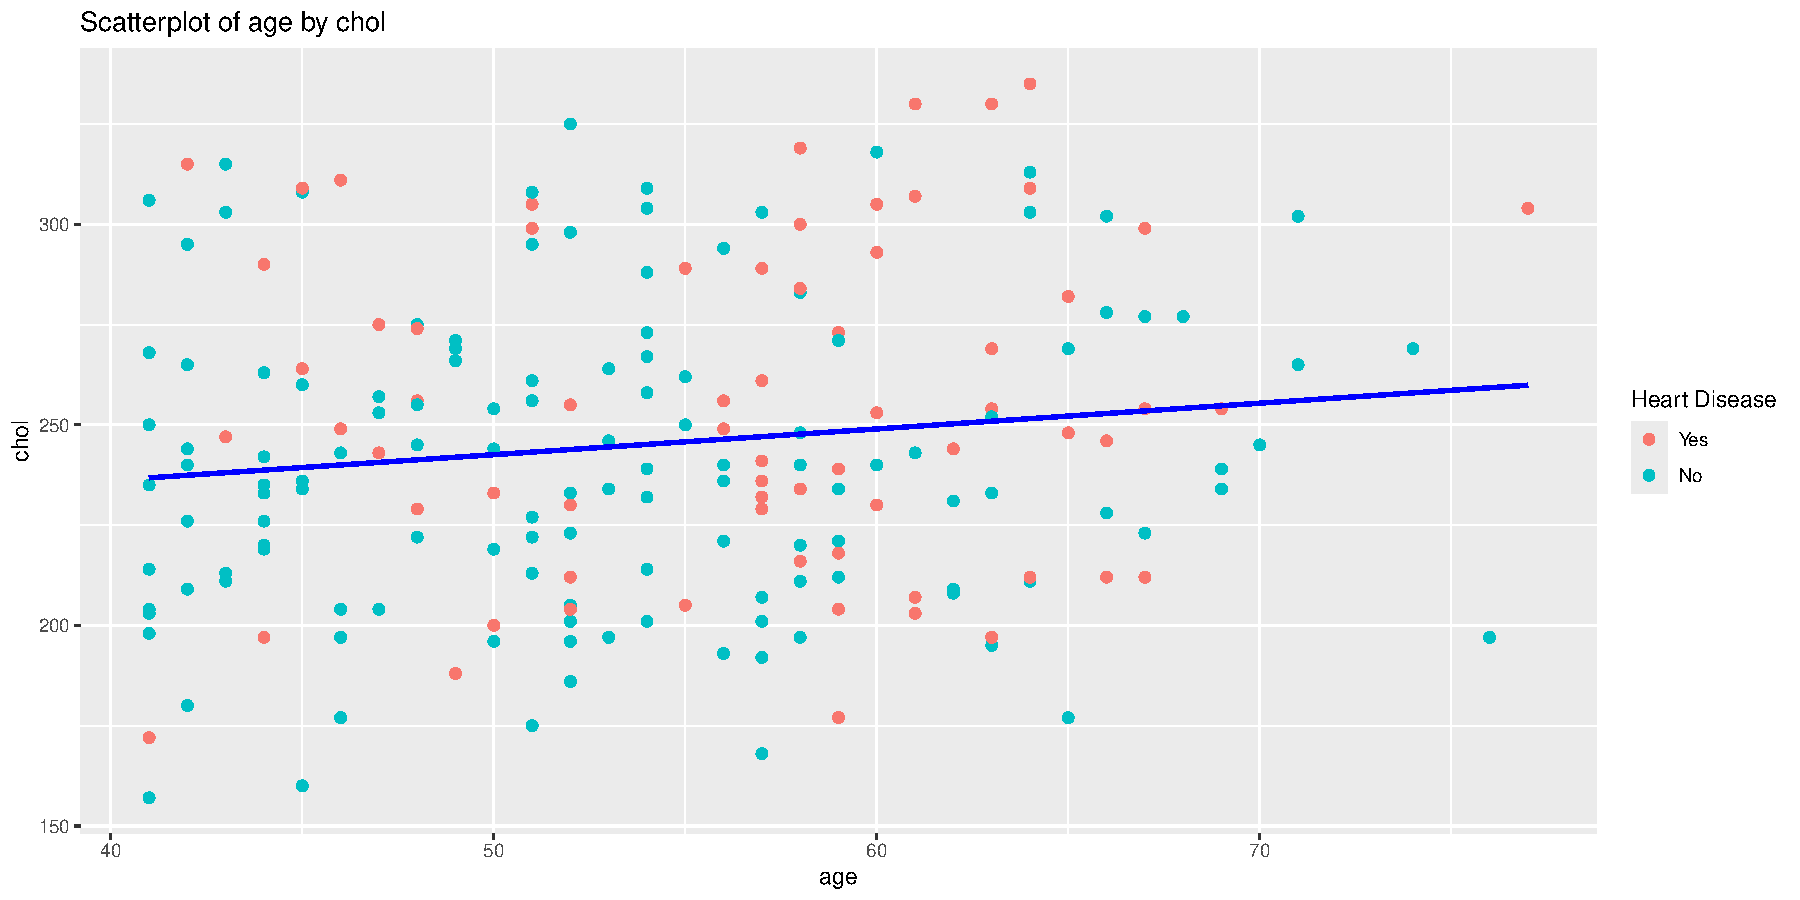
\includegraphics[keepaspectratio]{heart_disease_risks_files/figure-latex/unnamed-chunk-26-2.pdf}}

\begin{Shaded}
\begin{Highlighting}[]
\FunctionTok{HeartDiseaseScatter}\NormalTok{(}\StringTok{"age"}\NormalTok{, }\StringTok{"trestbps"}\NormalTok{)}
\end{Highlighting}
\end{Shaded}

\pandocbounded{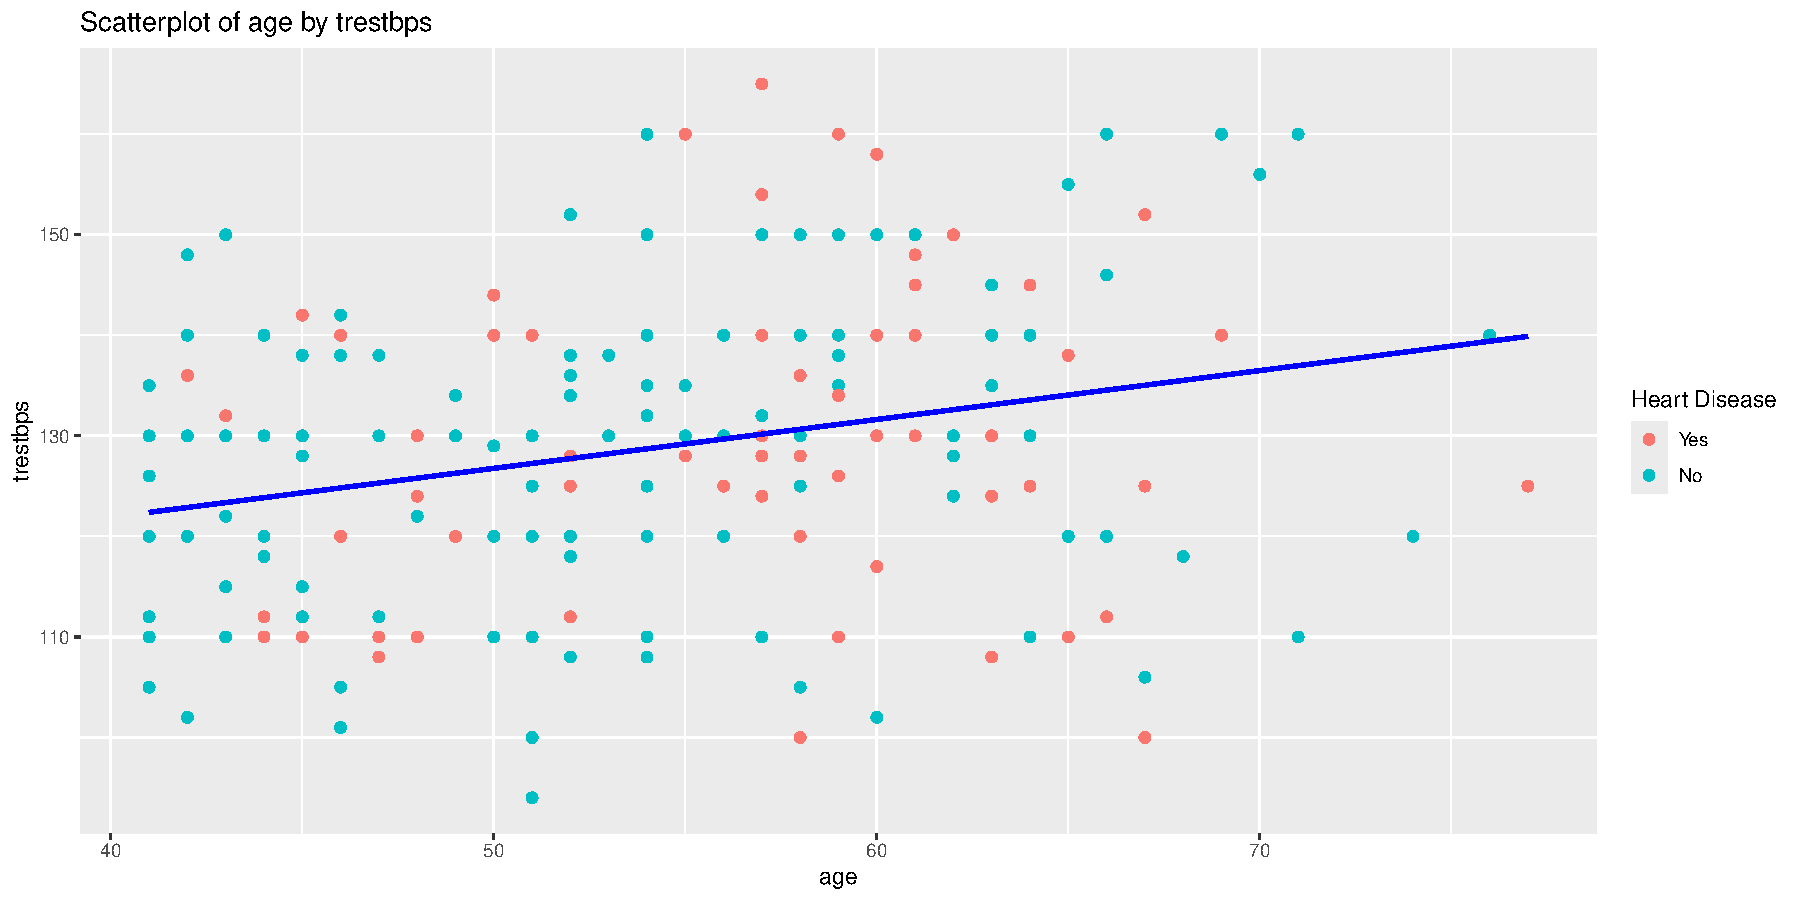
\includegraphics[keepaspectratio]{heart_disease_risks_files/figure-latex/unnamed-chunk-26-3.pdf}}

\begin{Shaded}
\begin{Highlighting}[]
\FunctionTok{HeartDiseaseScatter}\NormalTok{(}\StringTok{"age"}\NormalTok{, }\StringTok{"thalach"}\NormalTok{)}
\end{Highlighting}
\end{Shaded}

\pandocbounded{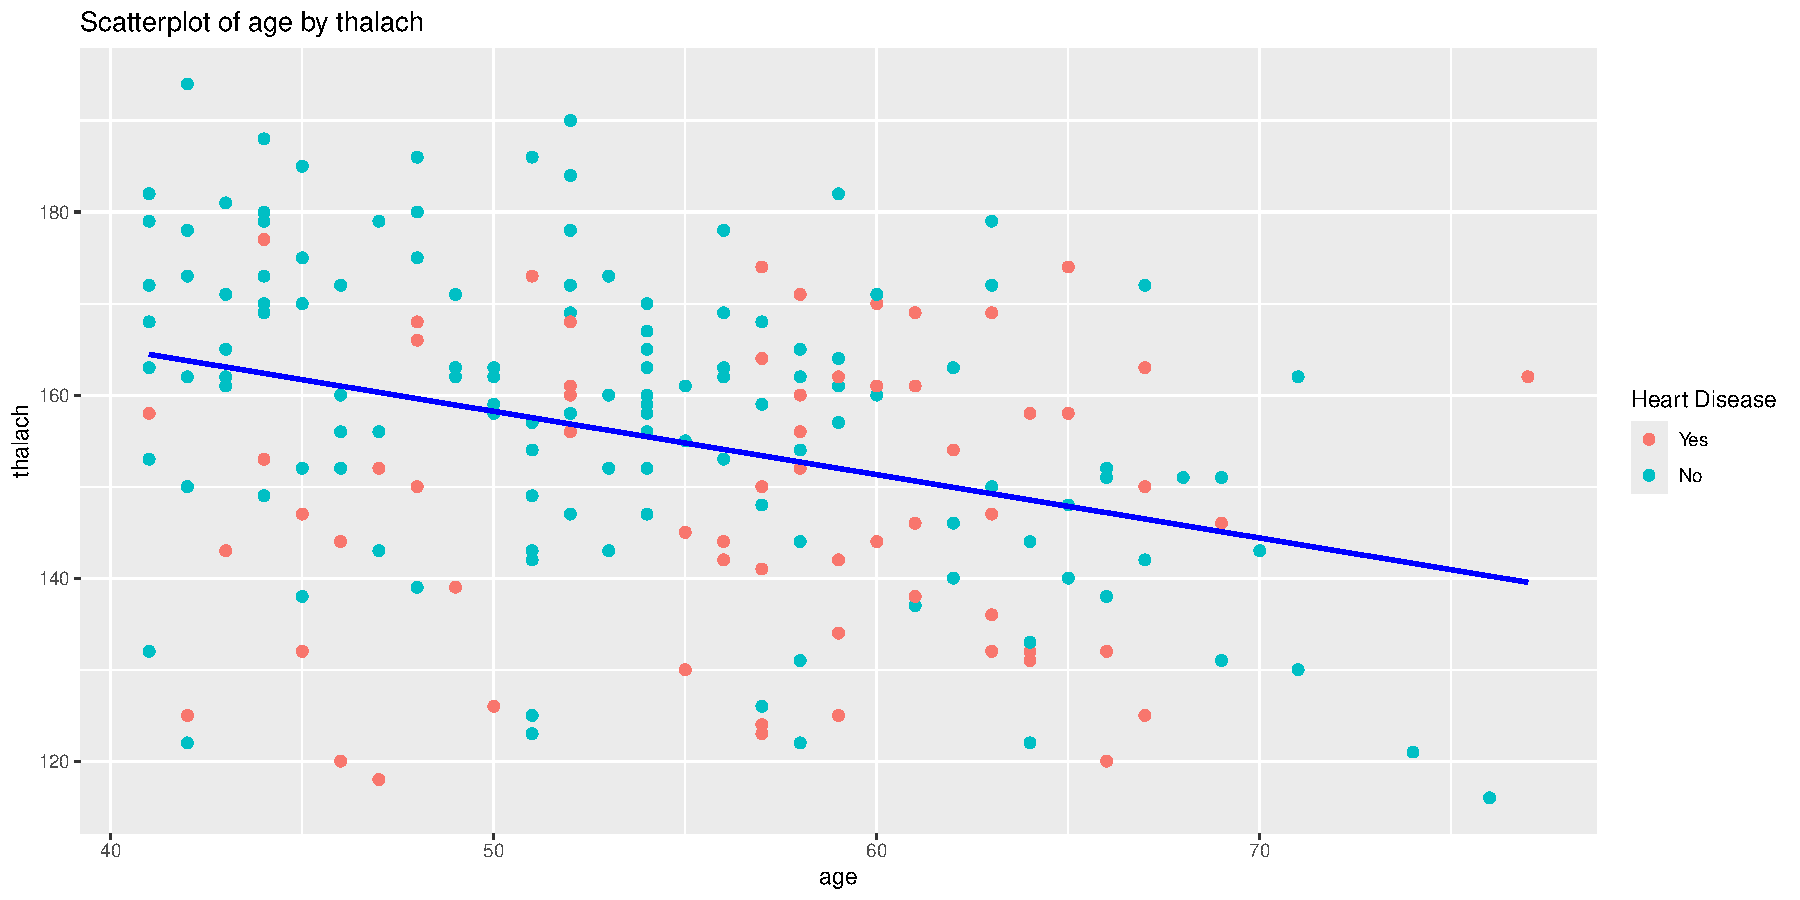
\includegraphics[keepaspectratio]{heart_disease_risks_files/figure-latex/unnamed-chunk-26-4.pdf}}

\begin{Shaded}
\begin{Highlighting}[]
\FunctionTok{HeartDiseaseScatter}\NormalTok{(}\StringTok{"chol"}\NormalTok{, }\StringTok{"thalach"}\NormalTok{)}
\end{Highlighting}
\end{Shaded}

\pandocbounded{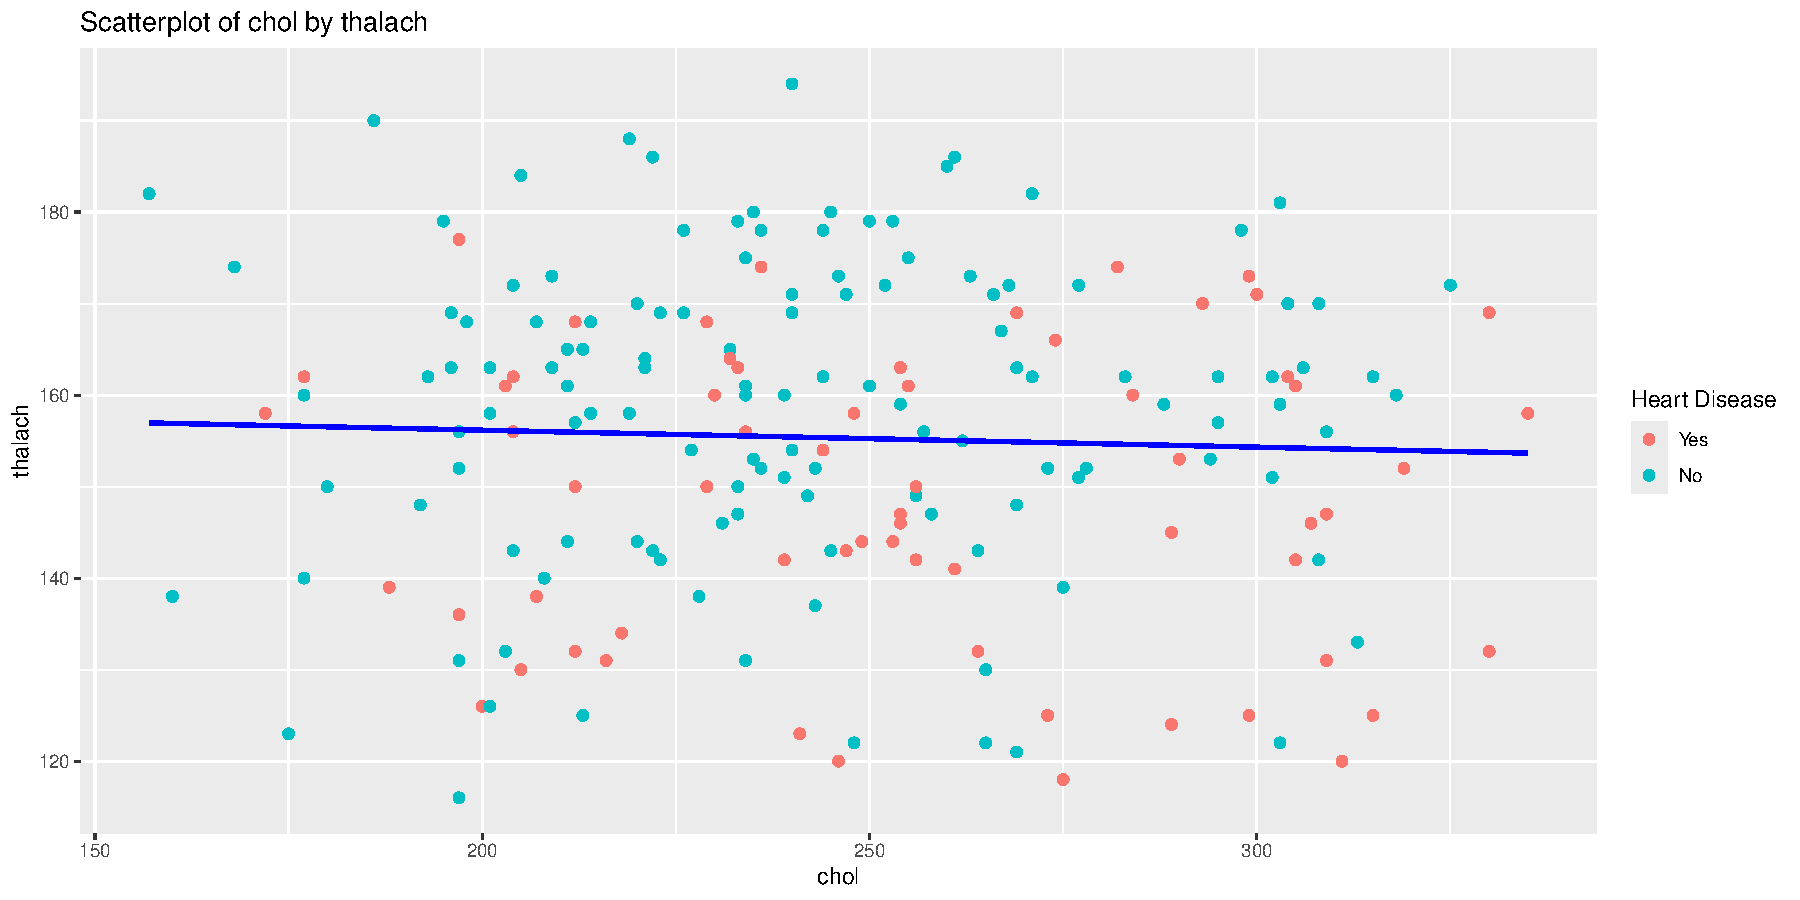
\includegraphics[keepaspectratio]{heart_disease_risks_files/figure-latex/unnamed-chunk-26-5.pdf}}

\begin{Shaded}
\begin{Highlighting}[]
\FunctionTok{HeartDiseaseScatter}\NormalTok{(}\StringTok{"trestbps"}\NormalTok{, }\StringTok{"chol"}\NormalTok{)}
\end{Highlighting}
\end{Shaded}

\pandocbounded{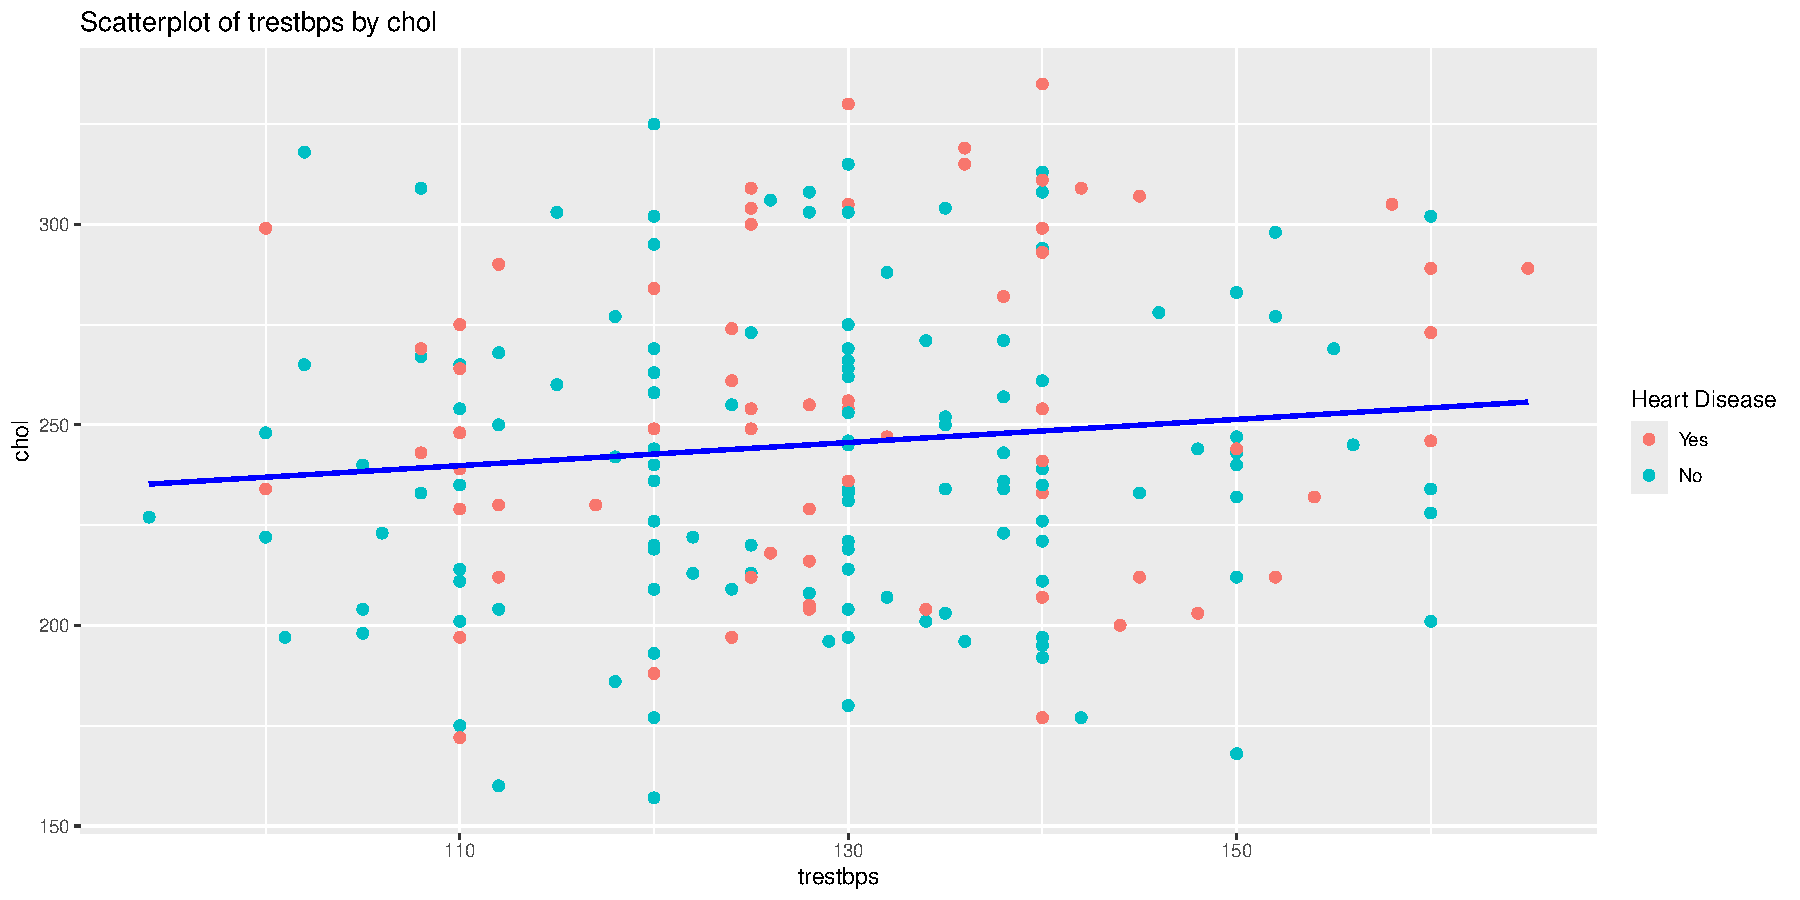
\includegraphics[keepaspectratio]{heart_disease_risks_files/figure-latex/unnamed-chunk-26-6.pdf}}

\begin{Shaded}
\begin{Highlighting}[]
\FunctionTok{HeartDiseaseScatter}\NormalTok{(}\StringTok{"thalach"}\NormalTok{, }\StringTok{"oldpeak"}\NormalTok{)}
\end{Highlighting}
\end{Shaded}

\pandocbounded{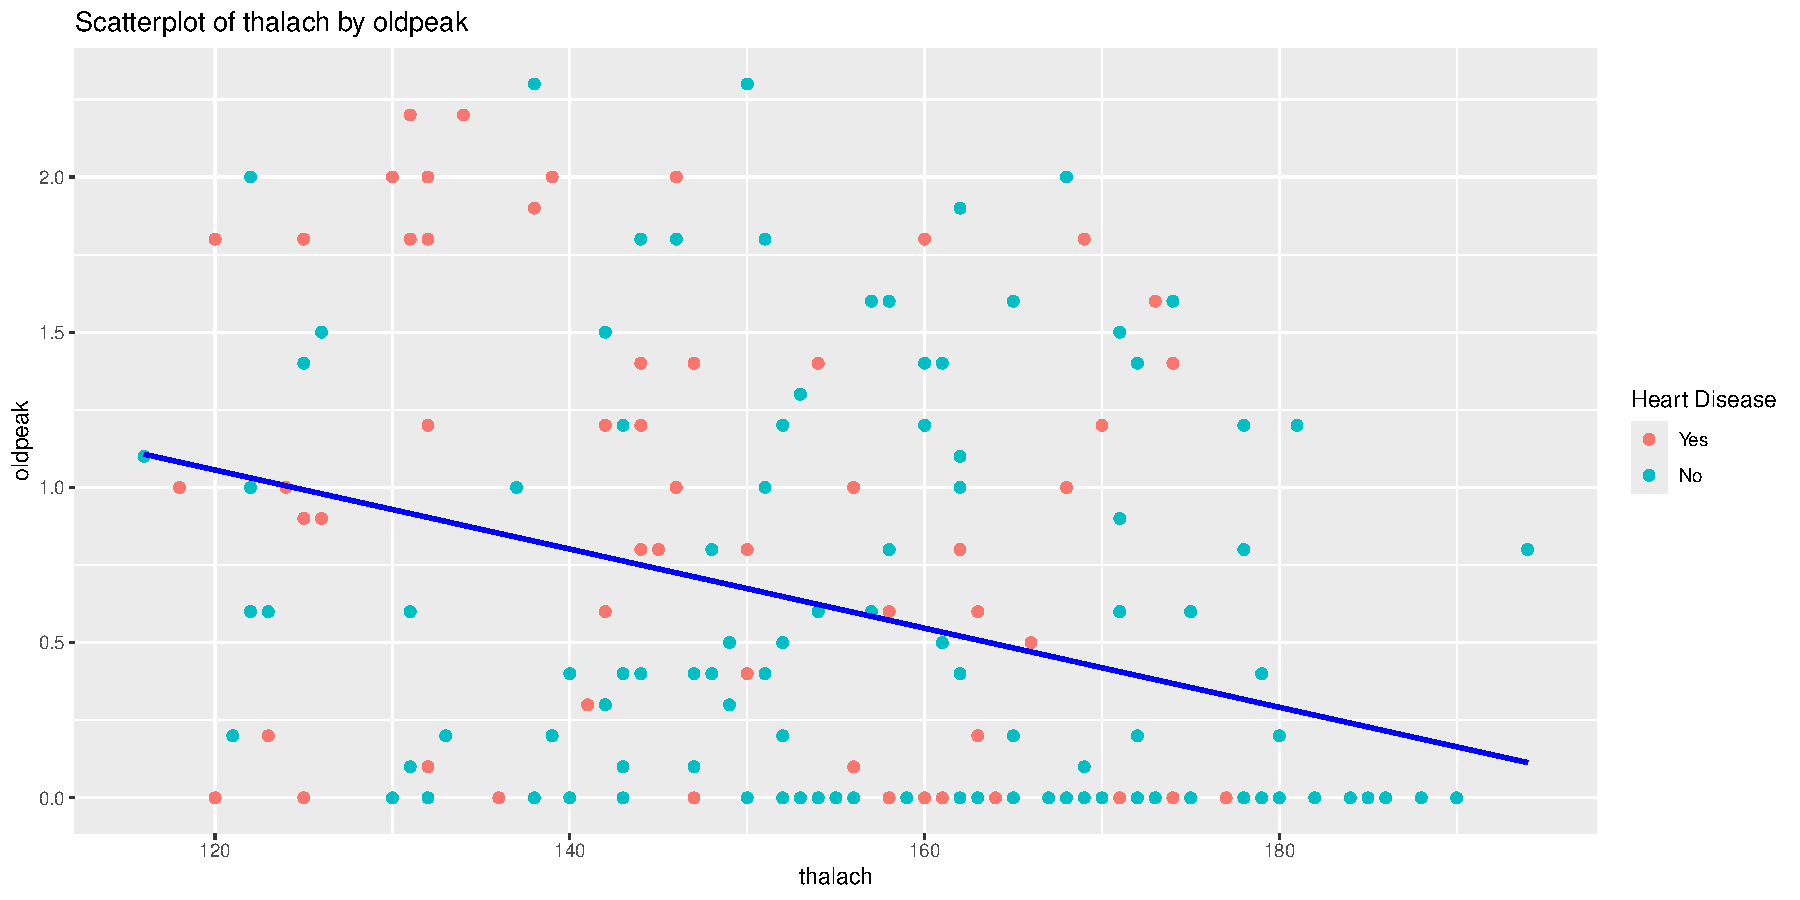
\includegraphics[keepaspectratio]{heart_disease_risks_files/figure-latex/unnamed-chunk-26-7.pdf}}

\subsubsection{Pairwise correlation
plots}\label{pairwise-correlation-plots}

Pairwise correlation plot for numerical variables

\begin{Shaded}
\begin{Highlighting}[]
\FunctionTok{ggpairs}\NormalTok{(Heart.df[, }\FunctionTok{c}\NormalTok{(}\StringTok{"age"}\NormalTok{, }\StringTok{"trestbps"}\NormalTok{, }\StringTok{"chol"}\NormalTok{, }
                     \StringTok{"thalach"}\NormalTok{, }\StringTok{"oldpeak"}\NormalTok{, }\StringTok{"target"}\NormalTok{)], }
        \FunctionTok{aes}\NormalTok{(}\AttributeTok{color =}\NormalTok{ target, }\AttributeTok{fill =}\NormalTok{ target))}
\end{Highlighting}
\end{Shaded}

\begin{verbatim}
## `stat_bin()` using `bins = 30`. Pick better value `binwidth`.
## `stat_bin()` using `bins = 30`. Pick better value `binwidth`.
## `stat_bin()` using `bins = 30`. Pick better value `binwidth`.
## `stat_bin()` using `bins = 30`. Pick better value `binwidth`.
## `stat_bin()` using `bins = 30`. Pick better value `binwidth`.
\end{verbatim}

\pandocbounded{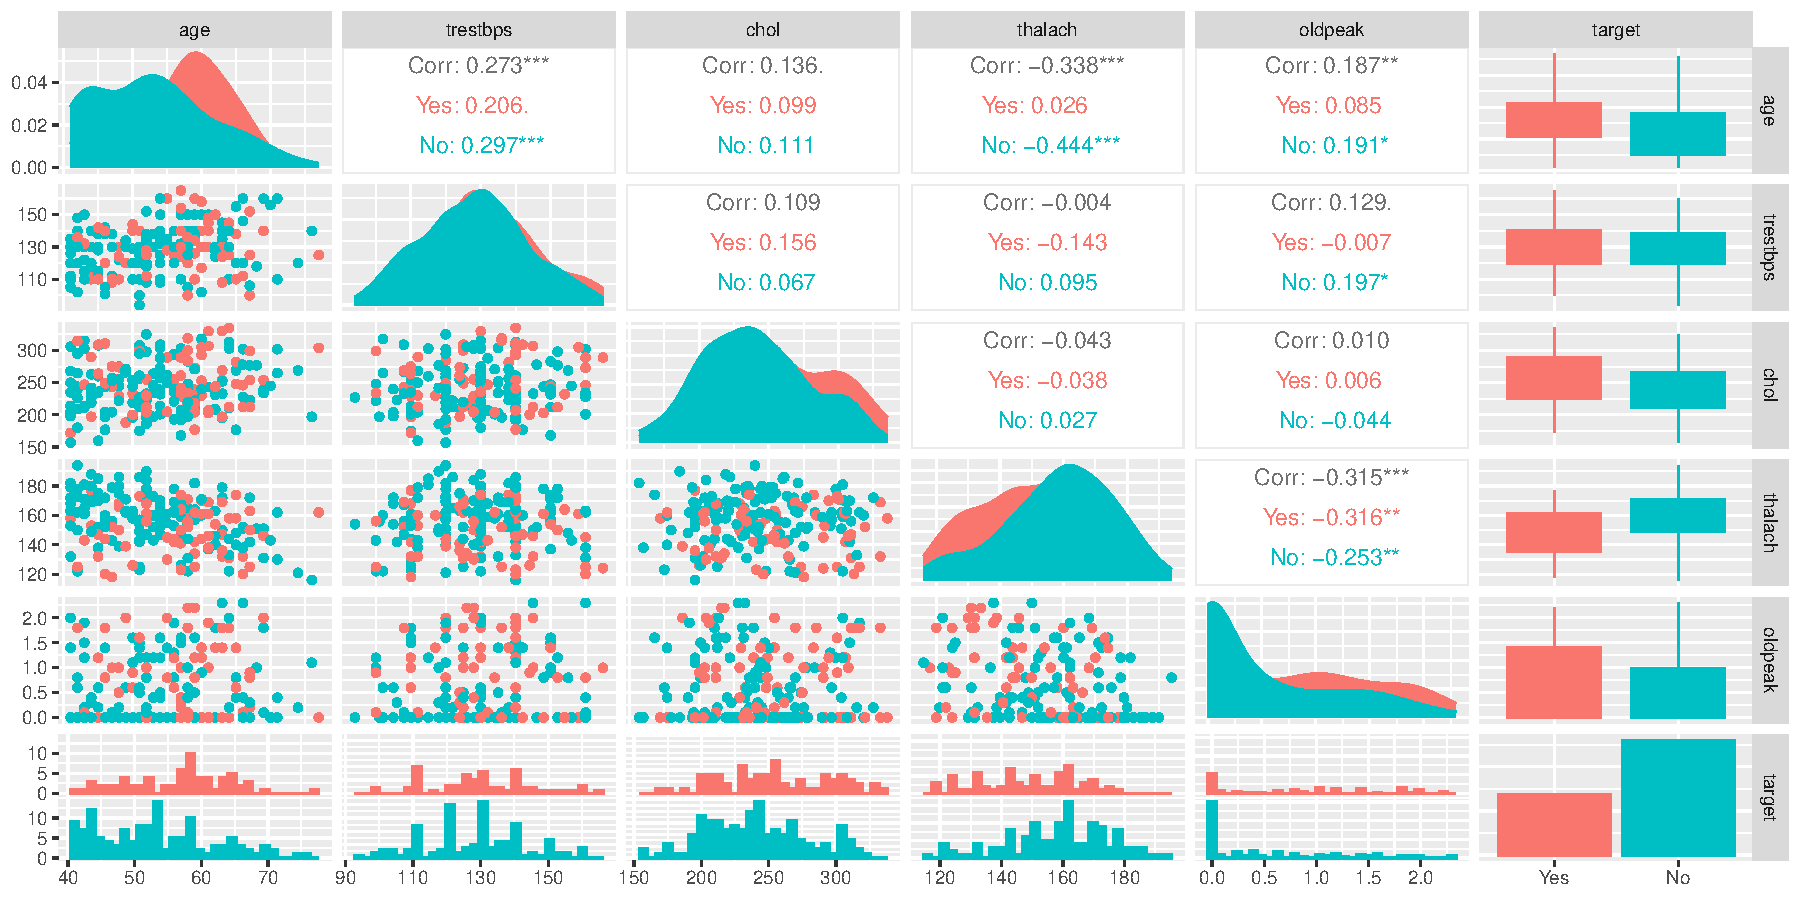
\includegraphics[keepaspectratio]{heart_disease_risks_files/figure-latex/unnamed-chunk-27-1.pdf}}

\subsubsection{Correlation matrix}\label{correlation-matrix}

Correlation matrix for numerical variables

\begin{Shaded}
\begin{Highlighting}[]
\CommentTok{\# Selecting only continuous variables}
\NormalTok{continuous\_vars }\OtherTok{\textless{}{-}} \FunctionTok{c}\NormalTok{(}\StringTok{"age"}\NormalTok{, }\StringTok{"trestbps"}\NormalTok{, }\StringTok{"chol"}\NormalTok{, }\StringTok{"thalach"}\NormalTok{, }\StringTok{"oldpeak"}\NormalTok{)}
\NormalTok{continuous\_data }\OtherTok{\textless{}{-}}\NormalTok{ Heart.df }\SpecialCharTok{\%\textgreater{}\%} \FunctionTok{select}\NormalTok{(}\FunctionTok{all\_of}\NormalTok{(continuous\_vars))}

\CommentTok{\# Calculating correlation matrix}
\NormalTok{correlation\_matrix }\OtherTok{\textless{}{-}} \FunctionTok{cor}\NormalTok{(continuous\_data)}

\CommentTok{\# Plotting the correlation matrix}
\FunctionTok{corrplot}\NormalTok{(correlation\_matrix, }\AttributeTok{method =} \StringTok{"circle"}\NormalTok{,}
         \AttributeTok{type =} \StringTok{"lower"}\NormalTok{, }\AttributeTok{tl.col =} \StringTok{"black"}\NormalTok{)}
\end{Highlighting}
\end{Shaded}

\pandocbounded{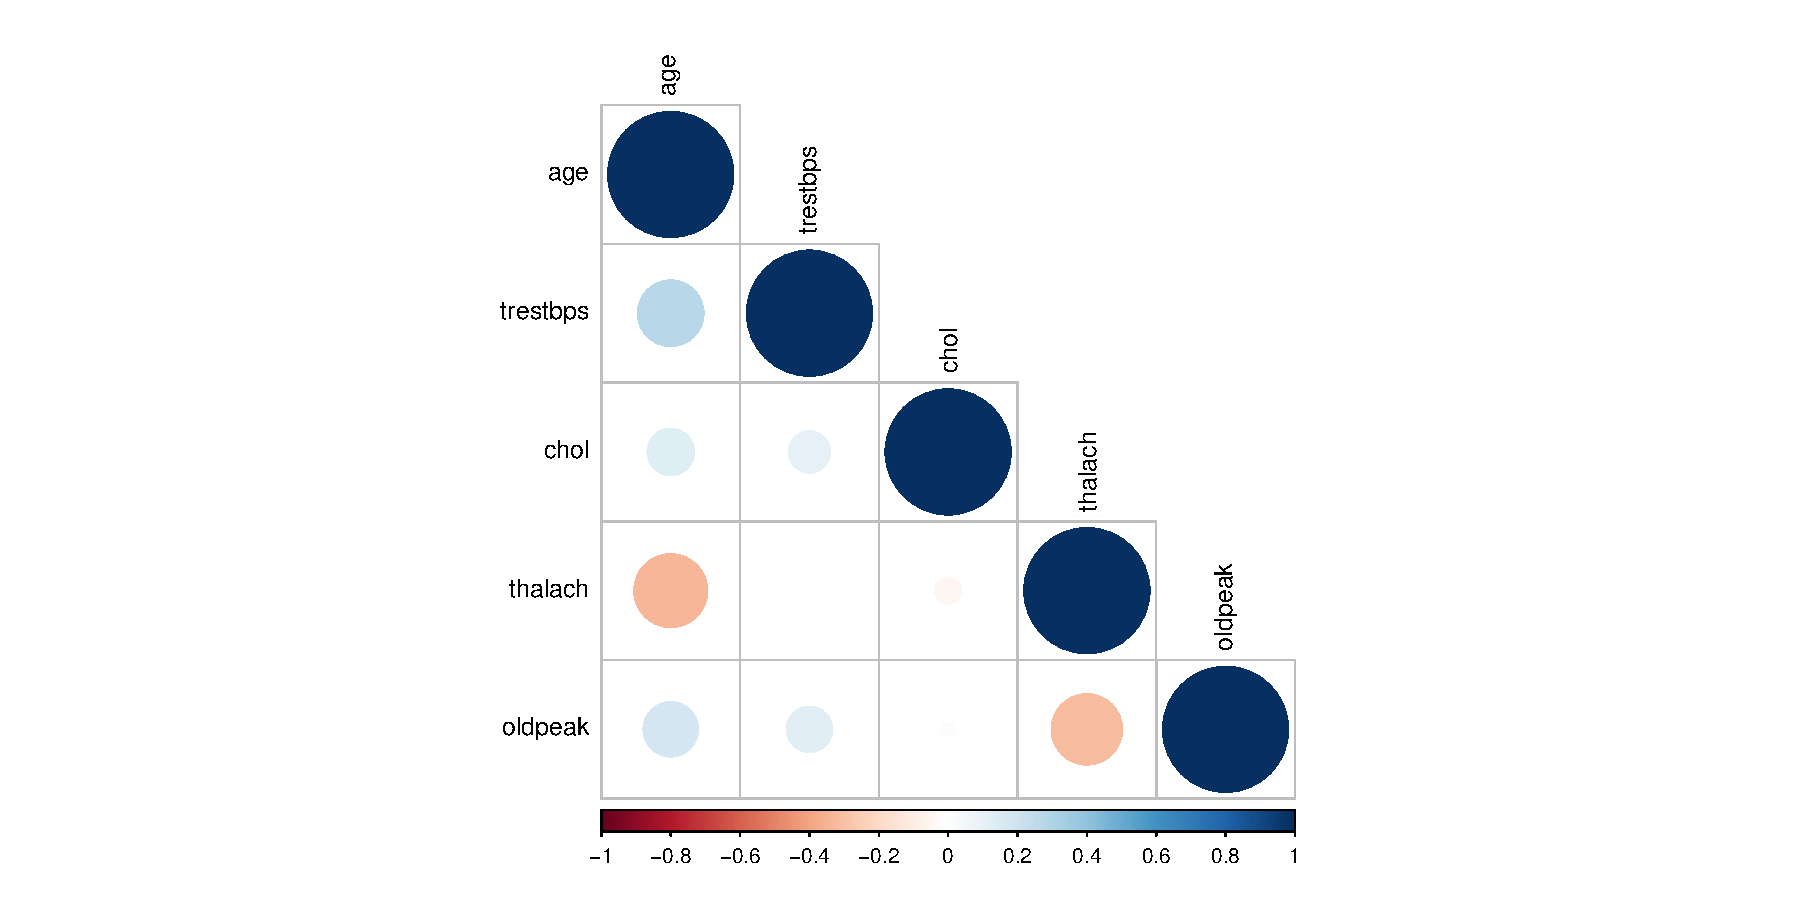
\includegraphics[keepaspectratio]{heart_disease_risks_files/figure-latex/unnamed-chunk-28-1.pdf}}

\subsubsection{Class imbalance}\label{class-imbalance}

\begin{Shaded}
\begin{Highlighting}[]
\NormalTok{Heart.df }\SpecialCharTok{\%\textgreater{}\%} \FunctionTok{count}\NormalTok{(target) }\SpecialCharTok{\%\textgreater{}\%} \FunctionTok{mutate}\NormalTok{(}\AttributeTok{pct =}\NormalTok{ n}\SpecialCharTok{/}\FunctionTok{sum}\NormalTok{(n))}
\end{Highlighting}
\end{Shaded}

\begin{verbatim}
##   target   n       pct
## 1    Yes  68 0.3434343
## 2     No 130 0.6565657
\end{verbatim}

\newpage

\section{\texorpdfstring{\textbf{Modeling}}{Modeling}}\label{modeling}

\newpage

\section{\texorpdfstring{\textbf{Evaluation}}{Evaluation}}\label{evaluation}

\newpage

\section{\texorpdfstring{\textbf{Deployment}}{Deployment}}\label{deployment}

\newpage

\section{\texorpdfstring{\textbf{Conclusion}}{Conclusion}}\label{conclusion}

\newpage

\section{\texorpdfstring{\textbf{Session
Information}}{Session Information}}\label{session-information}

\begin{Shaded}
\begin{Highlighting}[]
\FunctionTok{sessionInfo}\NormalTok{()}
\end{Highlighting}
\end{Shaded}

\begin{verbatim}
## R version 4.5.1 (2025-06-13)
## Platform: x86_64-apple-darwin20
## Running under: macOS Sequoia 15.7.1
## 
## Matrix products: default
## BLAS:   /Library/Frameworks/R.framework/Versions/4.5-x86_64/Resources/lib/libRblas.0.dylib 
## LAPACK: /Library/Frameworks/R.framework/Versions/4.5-x86_64/Resources/lib/libRlapack.dylib;  LAPACK version 3.12.1
## 
## locale:
## [1] en_US.UTF-8/en_US.UTF-8/en_US.UTF-8/C/en_US.UTF-8/en_US.UTF-8
## 
## time zone: America/Chicago
## tzcode source: internal
## 
## attached base packages:
## [1] stats     graphics  grDevices utils     datasets  methods   base     
## 
## other attached packages:
##  [1] pROC_1.19.0.1        GGally_2.4.0         corrplot_0.95       
##  [4] rpart_4.1.24         e1071_1.7-16         formatR_1.14        
##  [7] randomForest_4.7-1.2 caret_7.0-1          lattice_0.22-7      
## [10] RCurl_1.98-1.17      lubridate_1.9.4      forcats_1.0.1       
## [13] stringr_1.5.2        dplyr_1.1.4          purrr_1.1.0         
## [16] readr_2.1.5          tidyr_1.3.1          tibble_3.3.0        
## [19] ggplot2_4.0.0        tidyverse_2.0.0     
## 
## loaded via a namespace (and not attached):
##  [1] tidyselect_1.2.1     timeDate_4041.110    farver_2.1.2        
##  [4] S7_0.2.0             bitops_1.0-9         fastmap_1.2.0       
##  [7] digest_0.6.37        timechange_0.3.0     lifecycle_1.0.4     
## [10] survival_3.8-3       magrittr_2.0.4       compiler_4.5.1      
## [13] rlang_1.1.6          tools_4.5.1          yaml_2.3.10         
## [16] data.table_1.17.8    knitr_1.50           labeling_0.4.3      
## [19] plyr_1.8.9           RColorBrewer_1.1-3   withr_3.0.2         
## [22] nnet_7.3-20          grid_4.5.1           stats4_4.5.1        
## [25] future_1.67.0        globals_0.18.0       scales_1.4.0        
## [28] iterators_1.0.14     MASS_7.3-65          tinytex_0.57        
## [31] cli_3.6.5            rmarkdown_2.30       generics_0.1.4      
## [34] rstudioapi_0.17.1    future.apply_1.20.0  reshape2_1.4.4      
## [37] tzdb_0.5.0           proxy_0.4-27         splines_4.5.1       
## [40] parallel_4.5.1       vctrs_0.6.5          hardhat_1.4.2       
## [43] Matrix_1.7-4         hms_1.1.3            listenv_0.9.1       
## [46] foreach_1.5.2        gower_1.0.2          recipes_1.3.1       
## [49] glue_1.8.0           parallelly_1.45.1    ggstats_0.11.0      
## [52] codetools_0.2-20     stringi_1.8.7        gtable_0.3.6        
## [55] pillar_1.11.1        htmltools_0.5.8.1    ipred_0.9-15        
## [58] lava_1.8.1           R6_2.6.1             evaluate_1.0.5      
## [61] class_7.3-23         Rcpp_1.1.0           nlme_3.1-168        
## [64] prodlim_2025.04.28   mgcv_1.9-3           xfun_0.53           
## [67] pkgconfig_2.0.3      ModelMetrics_1.2.2.2
\end{verbatim}

\end{document}
